%% chapter04_slides.tex
%% Heuristics for the Vehicle Routing Problem
%% Based on: Laporte, Ropke, Vidal — Chapter 4 of
%%   "Vehicle Routing: Problems, Methods, and Applications" (2nd ed., SIAM 2014)
%% Self-contained lecture-note style slides (reader-friendly, no presenter needed)
\documentclass[aspectratio=169,10pt]{beamer}

\usetheme{Madrid}
\usecolortheme{seahorse}
\setbeamertemplate{footline}[frame number]
\setbeamertemplate{navigation symbols}{}

\usepackage{amsmath,amssymb,amsthm}
\usepackage{booktabs}
\usepackage{array}
\usepackage{graphicx}
\usepackage{xcolor}
\usepackage{listings}
\usepackage{multicol}
\usepackage{tikz}
\usetikzlibrary{arrows.meta,positioning,shapes.geometric}

\graphicspath{{figures/}}

\lstset{
  language=Python,
  basicstyle=\ttfamily\scriptsize,
  numbers=left,
  numberstyle=\tiny\color{gray},
  frame=single,
  backgroundcolor=\color{gray!7},
  commentstyle=\color{green!50!black}\itshape,
  keywordstyle=\color{blue!80!black}\bfseries,
  stringstyle=\color{orange!70!black},
  breaklines=true,
  tabsize=4,
  showstringspaces=false,
}

% ─── title page ───────────────────────────────────────────────────────────────
\title[Ch.4: Heuristics for VRP]{%
  Chapter 4: Heuristics for the Vehicle Routing Problem}
\subtitle{\textit{Vehicle Routing: Problems, Methods, and Applications}\\
  2nd edition, SIAM 2014}
\author{Gilbert Laporte \and Stefan Ropke \and Thibaut Vidal}
\date{Slides prepared for independent study}
\institute{SIAM Monographs on Discrete Mathematics and Applications}

% ─── document ─────────────────────────────────────────────────────────────────
\begin{document}

\begin{frame}
  \titlepage
\end{frame}

% ──────────────────────────────────────────────────────────────────────────────
\begin{frame}[allowframebreaks]{Table of Contents}
  \tableofcontents
\end{frame}

% ══════════════════════════════════════════════════════════════════════════════
\section{Introduction}
% ══════════════════════════════════════════════════════════════════════════════

\begin{frame}[allowframebreaks]{Introduction: Why Heuristics?}

  The Vehicle Routing Problem (VRP) in its most basic form asks for a set
  of minimum-cost routes, all starting and ending at a common \emph{depot},
  that collectively visit a given set of customers while respecting vehicle
  capacity constraints.  Because the VRP is NP-hard, exact algorithms can
  solve instances with only a few hundred customers within reasonable time
  limits.  Real-world logistics instances often contain thousands of
  customers, making exact methods computationally infeasible.

  \begin{block}{The Role of Heuristics}
    A \textbf{heuristic} is an algorithm that sacrifices the guarantee of
    finding an optimal solution in favour of finding a good solution quickly.
    For the VRP, state-of-the-art heuristics routinely produce solutions
    within \textbf{0.5\%} of the best known optimum on standard benchmark
    instances, at a fraction of the computational cost of exact methods.
  \end{block}

  The evolution of VRP heuristics spans more than five decades.  The first
  practical heuristic --- the Clarke-Wright savings algorithm --- was
  published in 1964.  Since the 1990s, \textbf{metaheuristics} (Tabu
  Search, Simulated Annealing, Genetic Algorithms, Ant Colony Optimisation,
  Large Neighbourhood Search) have superseded classical improvement
  procedures as the dominant paradigm, and recent \textbf{hybrid} and
  \textbf{unified} algorithms combine strengths from several frameworks.

  \framebreak

  \begin{block}{Three Broad Categories}
    \begin{enumerate}
      \item \textbf{Constructive heuristics} build a feasible solution from
        scratch, inserting customers one at a time or merging routes
        incrementally.  They are fast but produce solutions of moderate
        quality.
      \item \textbf{Classical improvement heuristics} start from an initial
        feasible solution and apply local-search moves (edge swaps,
        customer relocations) to reduce its cost.  They refine
        constructive solutions but may get stuck in local optima.
      \item \textbf{Metaheuristics} guide the search over a much wider
        neighbourhood, accepting worsening moves (temporarily or
        probabilistically) to escape local optima.  They achieve the best
        solution quality but require more computation time.
    \end{enumerate}
  \end{block}

  \begin{alertblock}{Key Takeaway}
    Modern practice typically chains these three levels: a constructive
    heuristic provides an initial solution, local-search operators improve
    it, and a metaheuristic framework orchestrates the overall search.
  \end{alertblock}

\end{frame}

% ══════════════════════════════════════════════════════════════════════════════
\section{Constructive Heuristics}
% ══════════════════════════════════════════════════════════════════════════════

\begin{frame}[allowframebreaks]{Constructive Heuristics: Overview}

  Constructive heuristics build a feasible solution from scratch without
  performing any subsequent improvement.  Their appeal lies in speed:
  given $n$ customers they typically run in $O(n^2 \log n)$ time or
  better.  The three most important constructive heuristics for the CVRP
  are the \textbf{Clarke-Wright savings algorithm}, the
  \textbf{nearest-neighbour} heuristic, and the \textbf{sweep} algorithm.

  \begin{block}{Common Starting Point}
    All three methods begin with a trivial \emph{radial} solution: every
    customer $i$ is served by a dedicated vehicle that travels
    depot $\to$ $i$ $\to$ depot.  The total cost of this solution is
    $2\sum_{i=1}^{n} d_{0i}$, where $d_{0i}$ denotes the distance from
    the depot (node $0$) to customer $i$.  Each method then tries to
    reduce this cost by consolidating customers into multi-stop routes.
  \end{block}

\end{frame}

% ─── Clarke-Wright ────────────────────────────────────────────────────────────
\begin{frame}[allowframebreaks]{The Clarke-Wright Savings Algorithm (1964)}

  The Clarke-Wright savings algorithm, introduced by G.\ Clarke and
  J.\ W.\ Wright in 1964, is arguably the most influential VRP heuristic
  ever published.  The central idea is simple: if we merge the route
  \mbox{depot $\to$ $i$ $\to$ depot} with the route
  \mbox{depot $\to$ $j$ $\to$ depot} into the single route
  \mbox{depot $\to$ $i$ $\to$ $j$ $\to$ depot}, we \emph{save}
  the two depot-return and depot-departure edges and instead pay for the
  direct edge between $i$ and $j$.

  \begin{block}{Savings Formula}
    The \textbf{saving} from combining customer $i$ and customer $j$ into
    the same route is defined as:
    \[
      s(i,j) = d_{0i} + d_{0j} - d_{ij}
    \]
    where $d_{0i}$ is the distance from the depot to customer $i$,
    $d_{0j}$ is the distance from the depot to customer $j$, and
    $d_{ij}$ is the direct distance between customers $i$ and $j$.
    A positive saving $s(i,j) > 0$ means that linking $i$ and $j$ reduces
    total travel distance.
  \end{block}

  The algorithm greedily merges routes in order of decreasing savings,
  subject to two feasibility conditions: (1)~the merge must not violate
  vehicle capacity, and (2)~$i$ and $j$ must currently be at the
  \emph{interior endpoints} of their respective routes (i.e., the
  customers that are directly adjacent to the depot).

  \framebreak

  \begin{block}{Clarke-Wright Parallel Algorithm}
    \begin{enumerate}
      \item Compute saving $s(i,j)$ for every pair $(i,j)$ with $i \ne j$.
      \item Sort all pairs in \textbf{decreasing} order of $s(i,j)$.
      \item Start with $n$ single-customer routes
            (depot $\to$ $i$ $\to$ depot for each $i$).
      \item For each pair $(i,j)$ in sorted order, \textbf{merge} the route
            ending at $i$ with the route beginning at $j$ into a single
            route, provided:
        \begin{itemize}
          \item $i$ and $j$ belong to \emph{different} current routes,
          \item $i$ is the last customer before the depot in its route,
          \item $j$ is the first customer after the depot in its route,
          \item The combined load does not exceed the vehicle capacity~$Q$.
        \end{itemize}
      \item Repeat until no more merges are feasible.
    \end{enumerate}
  \end{block}

  \begin{exampleblock}{Worked Example: 4 Customers, $Q = 10$}
    Suppose the depot is at origin $(0,0)$ and four customers are located
    at $c_1=(3,0)$, $c_2=(5,0)$, $c_3=(0,3)$, $c_4=(0,5)$ with demands
    $q_1=q_2=q_3=q_4=3$ and Euclidean distances.  Then:
    \begin{align*}
      s(1,2) &= 3 + 5 - 2 = 6 \quad \text{(very profitable: both on same axis)}\\
      s(3,4) &= 3 + 5 - 2 = 6 \\
      s(1,3) &= 3 + 3 - \sqrt{18} \approx 1.76 \\
      s(2,4) &= 5 + 5 - \sqrt{50} \approx 2.93
    \end{align*}
    Merging $(1,2)$ first gives route D$\to$1$\to$2$\to$D (load $=6 \le 10$).
    Merging $(3,4)$ gives route D$\to$3$\to$4$\to$D (load $=6 \le 10$).
    Final solution: \textbf{two routes}, total distance $= 2+2+2+2+3+5= 16$
    vs.\ initial $2(3+5+3+5)=32$.  Savings $= 50\%$.
  \end{exampleblock}

  \framebreak

  \begin{center}
    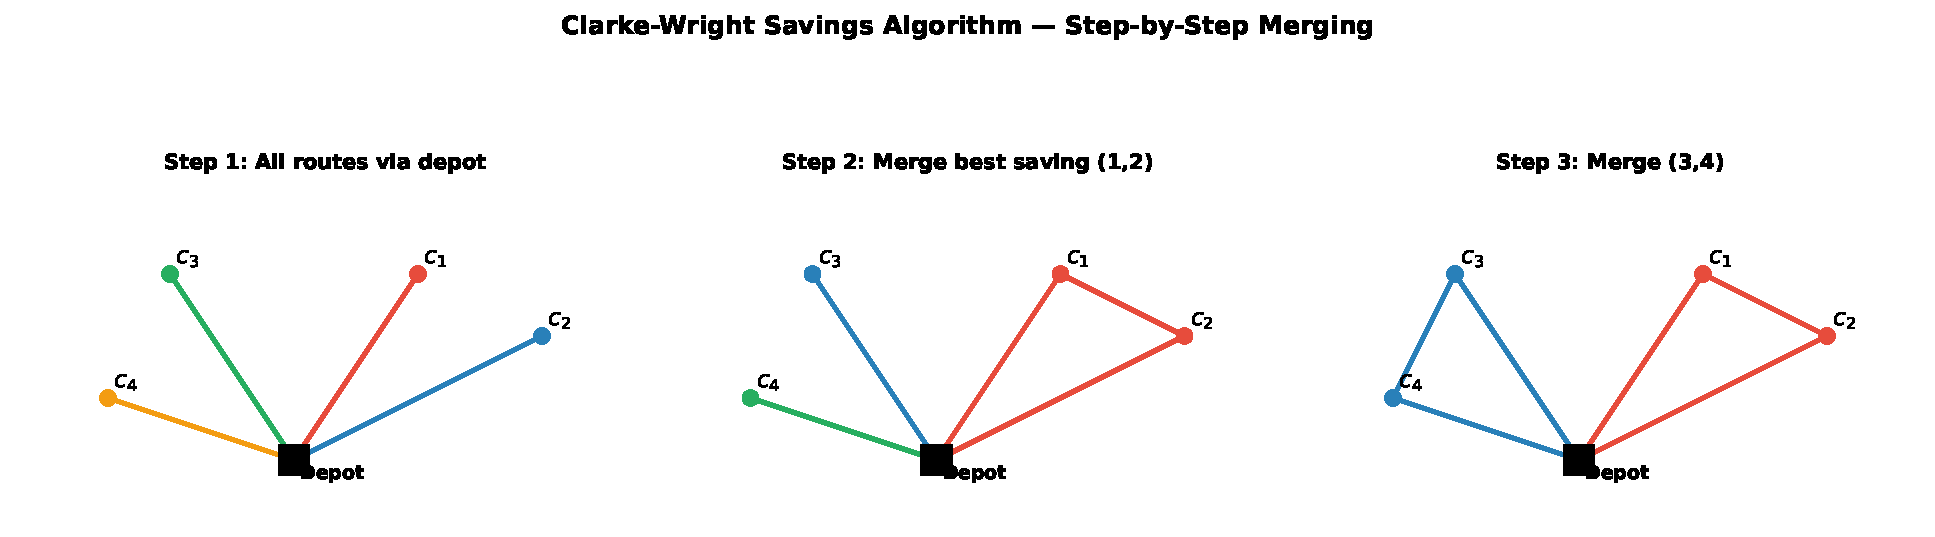
\includegraphics[width=0.95\textwidth]{cw_savings_steps.pdf}
  \end{center}

  \begin{alertblock}{Key Insight}
    The Clarke-Wright algorithm is greedy and does not backtrack.  It runs
    in $O(n^2 \log n)$ time (dominated by the sort of savings) and
    typically produces solutions \textbf{10--15\%} above the optimum.
    A \emph{sequential} variant processes savings one by one and extends
    a single active route; the \emph{parallel} variant (shown above)
    builds all routes simultaneously and generally gives better results.
  \end{alertblock}

\end{frame}

% ─── Nearest Neighbour ────────────────────────────────────────────────────────
\begin{frame}[allowframebreaks]{Nearest Neighbour Heuristic}

  The nearest-neighbour (NN) heuristic is one of the simplest constructive
  methods for the Travelling Salesman Problem and is easily adapted to the
  VRP.  The idea is to mimic how a driver naturally plans a delivery
  tour: at each step, visit the \emph{closest unvisited customer} that
  can be reached without violating the vehicle's capacity constraint.

  \begin{block}{Nearest Neighbour Algorithm for CVRP}
    \begin{enumerate}
      \item Set current position $\leftarrow$ depot; remaining capacity
            $\leftarrow Q$; all customers unvisited.
      \item While unvisited customers remain:
        \begin{enumerate}
          \item[(a)] Among all unvisited customers $j$ with demand
                $q_j \le$ remaining capacity, select the one with
                minimum distance $d(\text{current}, j)$.
          \item[(b)] If no such customer exists, return to the depot and
                start a new route (reset remaining capacity to $Q$).
          \item[(c)] Otherwise, append $j$ to the current route; update
                current position and remaining capacity.
        \end{enumerate}
      \item Return all vehicles to the depot.
    \end{enumerate}
  \end{block}

  \begin{center}
    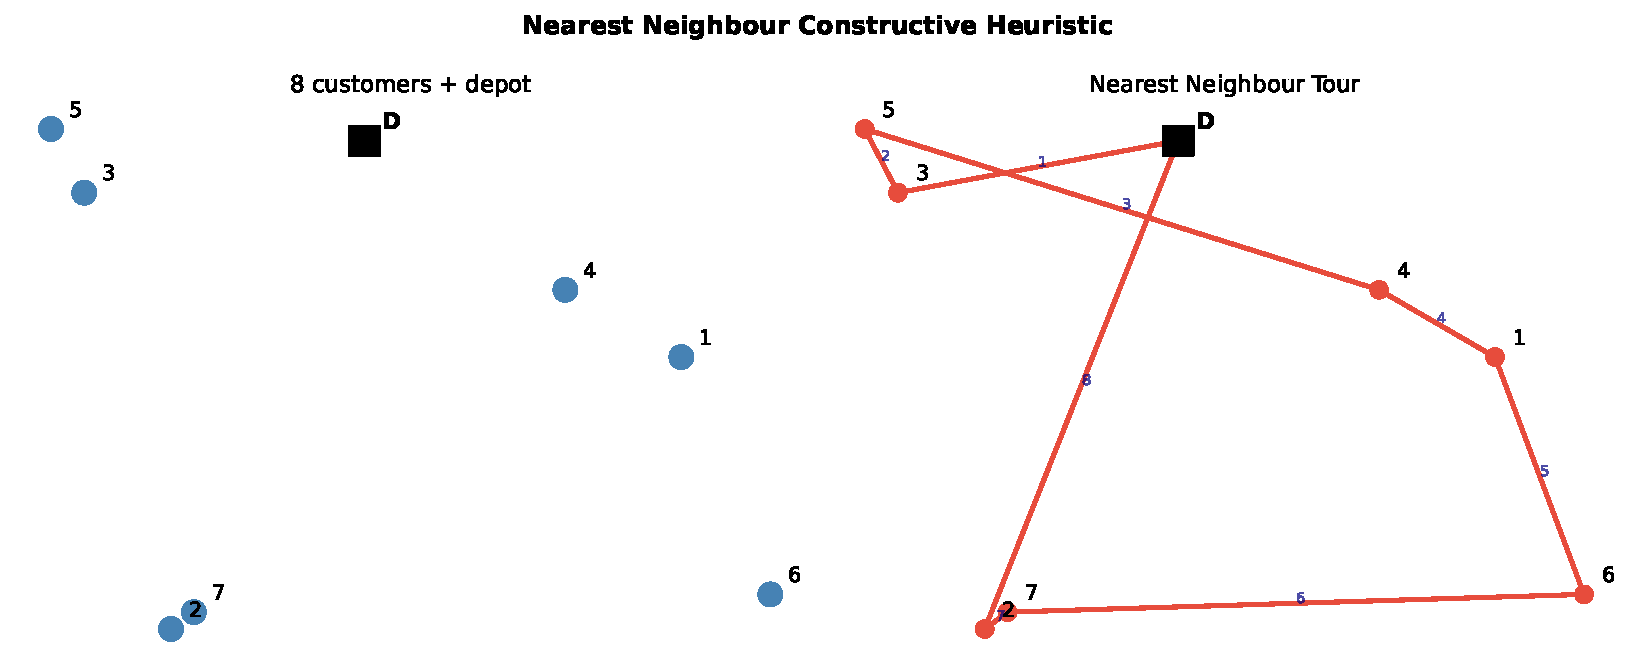
\includegraphics[width=0.7\textwidth]{nearest_neighbour.pdf}
  \end{center}

  \framebreak

  \begin{exampleblock}{Worked Example: 5 Customers}
    Customers at positions: $c_1=(1,1)$, $c_2=(3,2)$, $c_3=(2,4)$,
    $c_4=(5,1)$, $c_5=(4,3)$; depot at $(0,0)$; all demands $q_i=2$;
    $Q=6$ (3 customers per route).

    \medskip
    Route 1 starts at depot $(0,0)$.  Nearest unvisited: $c_1$ at
    distance $\sqrt{2}\approx 1.41$.  From $c_1$: nearest is $c_2$ at
    distance $\sqrt{(2^2+1^2)} = \sqrt{5} \approx 2.24$.  Remaining
    capacity after $c_1,c_2$: $6-4=2$, so one more customer fits.
    From $c_2$: nearest with demand $\le 2$ is $c_5$ at
    $\sqrt{(1^2+1^2)}=\sqrt{2}$.  Route full.  Return to depot.

    \medskip
    Route 2: nearest of $\{c_3,c_4\}$ from depot is $c_4$ at
    $\sqrt{26}\approx 5.1$.  From $c_4$: $c_3$ is at
    $\sqrt{9+9}\approx 4.24$.  Route full.  Return to depot.

    \medskip
    Final solution: Route 1: D$\to c_1 \to c_2 \to c_5\to$D;
    Route 2: D$\to c_4\to c_3\to$D.
  \end{exampleblock}

  \begin{alertblock}{Key Insight}
    The nearest-neighbour heuristic is very fast ($O(n^2)$) but produces
    solutions that can be 20--25\% above optimal, because greedily
    choosing the nearest neighbour early on may create expensive
    return trips later.  It is best used as a starting point for
    improvement procedures.
  \end{alertblock}

\end{frame}

% ─── Sweep ────────────────────────────────────────────────────────────────────
\begin{frame}[allowframebreaks]{Sweep Algorithm (Gillet \& Miller, 1974)}

  The sweep algorithm, introduced by Gillet and Miller in 1974, exploits
  the geometric structure of the VRP.  It converts the 2-D routing
  problem into a much simpler 1-D packing problem by representing each
  customer's position in polar coordinates centred at the depot.
  Customers are then clustered by \emph{sweeping} a ray from the depot
  in a fixed direction and grouping consecutive customers until the
  vehicle capacity is exhausted.

  \begin{block}{Sweep Algorithm}
    \begin{enumerate}
      \item Convert each customer $i$ to polar coordinates
            $(\rho_i, \theta_i)$ relative to the depot, where $\rho_i$
            is the distance and $\theta_i$ is the angle.
      \item Sort customers by angle $\theta_i$ (breaking ties by distance).
      \item Rotate a sweep line counterclockwise starting from angle
            $\theta_{\min}$.  Assign customers to the current vehicle in
            angular order until the capacity $Q$ would be exceeded;
            then close that route and start a new vehicle.
      \item Within each cluster, solve the single-vehicle TSP (or use a
            nearest-neighbour sub-tour) to determine the visit order.
    \end{enumerate}
  \end{block}

  \begin{center}
    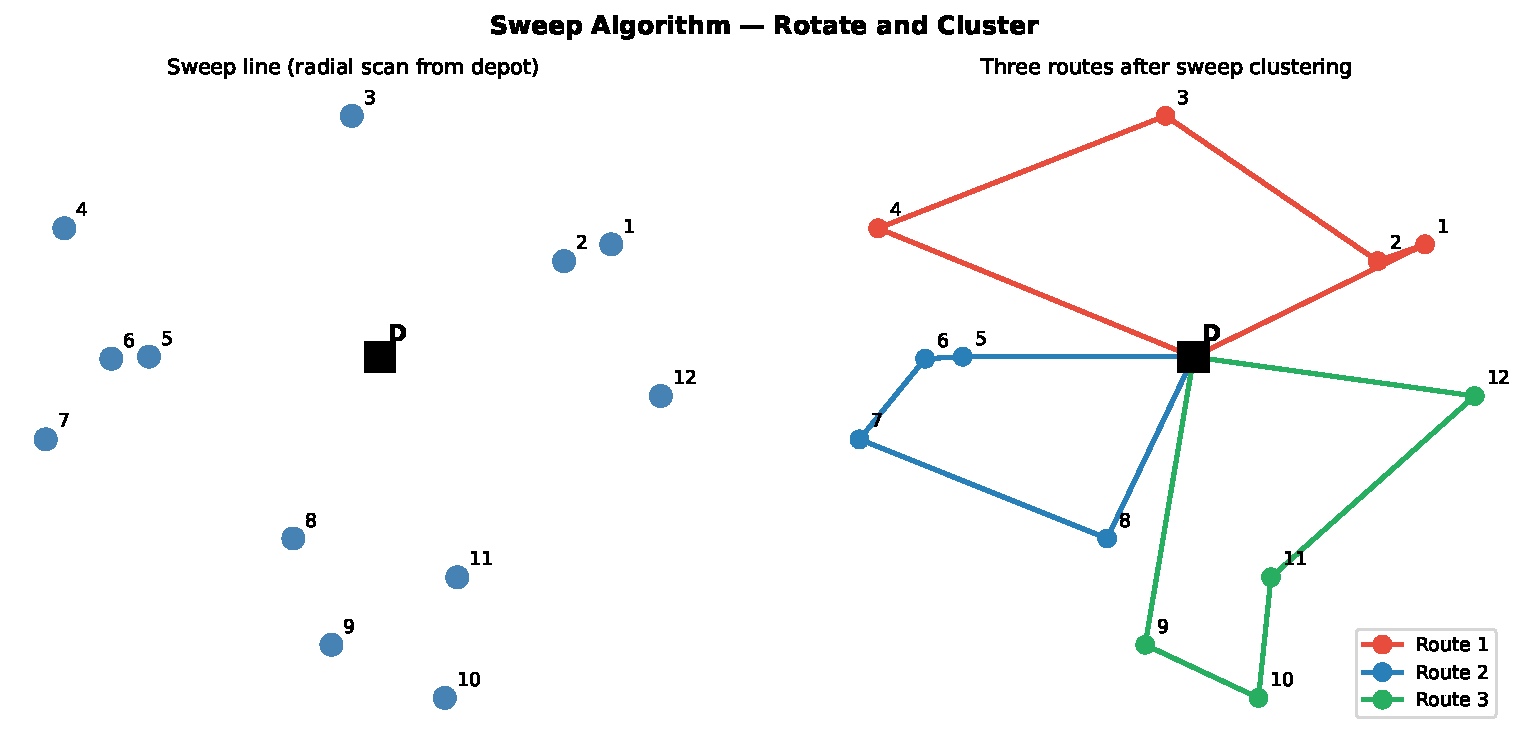
\includegraphics[width=0.7\textwidth]{sweep_algorithm.pdf}
  \end{center}

  \framebreak

  \begin{exampleblock}{Worked Example}
    Suppose 9 customers are sorted by angle: $\theta_1 < \theta_2 < \cdots
    < \theta_9$, with demands all equal to 3 and $Q=9$.  The sweep groups
    customers $\{1,2,3\}$ into Route~1 (total demand $=9$, exactly at
    capacity), $\{4,5,6\}$ into Route~2, and $\{7,8,9\}$ into Route~3.
    Each route's visit order is then determined by solving the small TSP
    on its 3 customers.
  \end{exampleblock}

  \begin{alertblock}{Key Insight}
    The sweep algorithm is extremely fast and naturally produces compact,
    geographically clustered routes.  Its main weakness is that the
    quality of the cluster-first, route-second decomposition depends on
    the starting angle; running the sweep from multiple starting angles
    and keeping the best result significantly improves solution quality.
  \end{alertblock}

\end{frame}

% ══════════════════════════════════════════════════════════════════════════════
\section{Classical Improvement Heuristics}
% ══════════════════════════════════════════════════════════════════════════════

\begin{frame}[allowframebreaks]{Classical Improvement Heuristics: Overview}

  Classical improvement heuristics (also called \emph{local search}
  methods) start from a feasible solution and iteratively apply
  \emph{moves} that replace the current solution with a better neighbour.
  A \textbf{move} is a small, reversible change to the solution (e.g.,
  swapping two edges, relocating one customer).  The algorithm terminates
  at a \textbf{local optimum}: a solution from which no single move
  produces an improvement.

  \begin{block}{General Local-Search Framework}
    \textbf{Input:} initial feasible solution $s_0$ \\
    \textbf{Repeat:}
    \begin{itemize}
      \item Enumerate all moves in the neighbourhood $\mathcal{N}(s)$.
      \item If a move $m$ exists such that $c(s \oplus m) < c(s)$, apply
            the \emph{best} (or first) improving move: $s \leftarrow s \oplus m$.
    \end{itemize}
    \textbf{Until} no improving move exists.  \\
    \textbf{Return} $s$.
  \end{block}

  The key design choices are the \textbf{neighbourhood structure}
  (which moves are considered) and the \textbf{pivot rule} (best-improving
  vs.\ first-improving).  Common VRP neighbourhood operators are
  2-opt, 3-opt, Or-opt, and the Lin-Kernighan move.

\end{frame}

% ─── 2-opt ────────────────────────────────────────────────────────────────────
\begin{frame}[allowframebreaks]{2-opt Local Search}

  The 2-opt move was introduced by Lin (1965) for the TSP and is the
  most widely used improvement operator.  The intuition is that an
  optimal tour should never have two \emph{crossing} edges, because
  uncrossing them always reduces the total distance.  A 2-opt move
  removes two edges from the current tour and reconnects the two
  resulting path segments in the only other feasible way.

  \begin{block}{2-opt Move Definition}
    Given a route $R = (v_0, v_1, \ldots, v_n, v_0)$ and two indices
    $1 \le i < j \le n$, the 2-opt move \textbf{removes} edges
    $(v_{i-1}, v_i)$ and $(v_j, v_{j+1})$ and \textbf{adds} edges
    $(v_{i-1}, v_j)$ and $(v_i, v_{j+1})$, which is equivalent to
    \textbf{reversing} the segment $v_i, v_{i+1}, \ldots, v_j$.

    The \textbf{improvement} from this move is:
    \[
      \Delta = d(v_{i-1}, v_i) + d(v_j, v_{j+1})
             - d(v_{i-1}, v_j) - d(v_i, v_{j+1})
    \]
    The move is applied whenever $\Delta > 0$ (i.e., the new edges are
    shorter than the old ones).
  \end{block}

  \begin{center}
    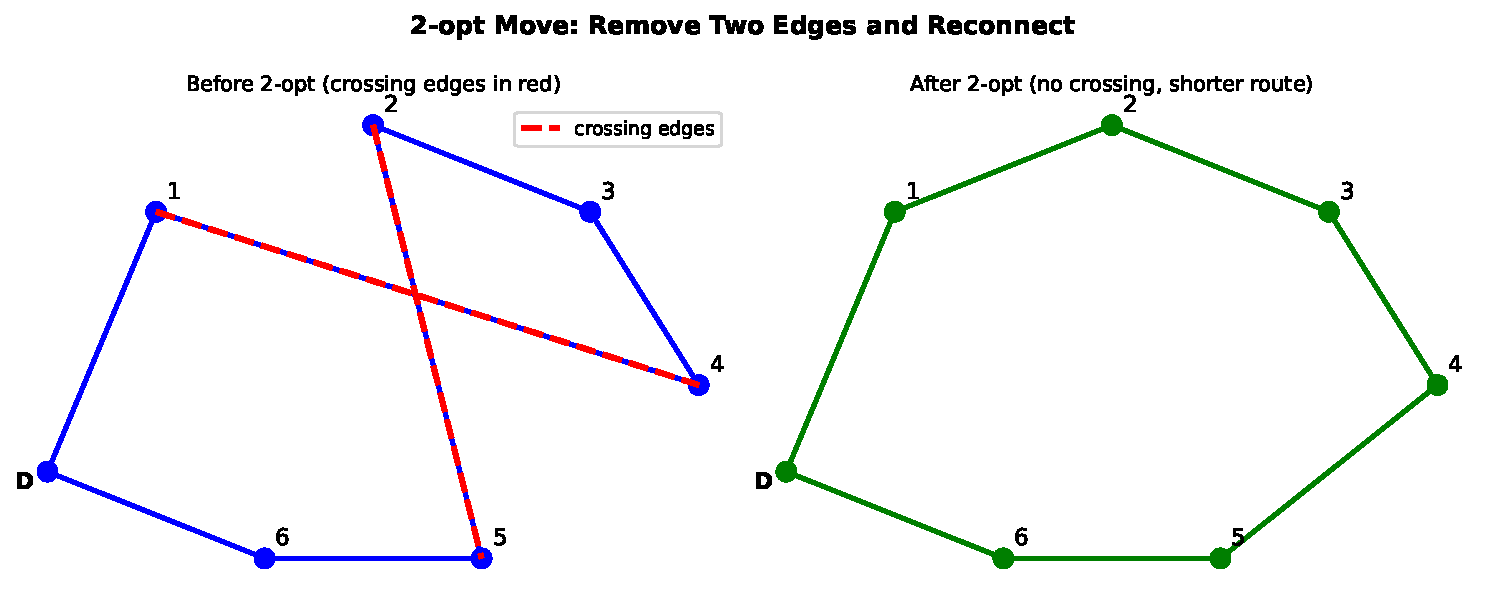
\includegraphics[width=0.7\textwidth]{two_opt.pdf}
  \end{center}

  \framebreak

  \begin{exampleblock}{Worked Example: 2-opt Improvement}
    Consider a single-route solution visiting customers in order
    1, 3, 5, 2, 4 with coordinates $c_1=(0,0)$, $c_2=(2,0)$,
    $c_3=(1,2)$, $c_4=(3,2)$, $c_5=(2,4)$ and depot at $(0,0)$.
    The current route D$\to$1$\to$3$\to$5$\to$2$\to$4$\to$D has a
    crossing between edges $(1,3)\to(5,2)$ and the path between $c_3$
    and $c_2$.  A 2-opt move on indices $i=2, j=4$ reverses the segment
    $3,5,2$ to $2,5,3$, giving route D$\to$1$\to$2$\to$5$\to$3$\to$4$\to$D,
    which removes the crossing and reduces the total distance.
  \end{exampleblock}

  \begin{alertblock}{Key Insight}
    The 2-opt neighbourhood has size $O(n^2)$.  A complete 2-opt pass
    over a route of length $n$ runs in $O(n^2)$ time.  The 2-opt local
    optimum is typically 5--10\% above the global optimum for random
    Euclidean instances.  For the VRP, 2-opt can also operate
    \emph{between} routes (intra-route and inter-route 2-opt).
  \end{alertblock}

\end{frame}

% ─── 3-opt / Lin-Kernighan ────────────────────────────────────────────────────
\begin{frame}[allowframebreaks]{3-opt and Lin-Kernighan Moves}

  The 3-opt move generalises 2-opt by removing \emph{three} edges and
  reconnecting the three resulting segments in the best possible way.
  There are 8 ways to reconnect 3 segments (including the original),
  and 3-opt considers all of them.  The Lin-Kernighan (LK) heuristic
  (1973) goes further and applies a \emph{variable-depth} search: it
  dynamically decides how many edges to exchange at each step,
  effectively exploring moves of order $k = 2, 3, 4, \ldots$ in a
  single sequential procedure.

  \begin{block}{3-opt: Three Edge Removal and Reconnection}
    Given a tour and three edge indices, remove edges
    $(v_{i-1}, v_i)$, $(v_{j-1}, v_j)$, $(v_{k-1}, v_k)$.
    The three resulting path segments can be reconnected in multiple
    ways.  The improvement $\Delta$ is computed for each reconnection,
    and the best improving reconnection is applied.
  \end{block}

  \begin{block}{Lin-Kernighan Variable-Depth Search}
    The LK algorithm starts by removing edge $(t_1, t_2)$ and
    sequentially adds a new edge $(t_2, t_3)$, removes the edge on
    the tour from $t_3$, adds the next edge, and so on, building a
    ``chain'' of improving candidate edges.  At each step it checks
    whether closing the chain (reconnecting the tour) gives an overall
    improvement.  The search terminates when no extension leads to
    improvement.  This sequential structure allows LK to efficiently
    discover many high-order moves that simpler $k$-opt methods would miss.
  \end{block}

  \begin{alertblock}{Key Insight}
    The LK heuristic for the TSP is one of the most powerful classical
    improvement methods, producing solutions typically within 1--2\% of
    optimal.  Its adaptation to the VRP (as part of LKH-style solvers)
    is more complex because feasibility (capacity) constraints must be
    maintained throughout the chain construction.
  \end{alertblock}

\end{frame}

% ─── Or-opt ────────────────────────────────────────────────────────────────────
\begin{frame}[allowframebreaks]{Or-opt: Customer Relocation}

  Or-opt moves, introduced by Or (1976), are a family of local-search
  operators that relocate a contiguous \emph{segment} of one or more
  customers from their current route to a different position (within the
  same route or in a different route).  Unlike 2-opt which reverses a
  segment, Or-opt keeps the segment's internal order intact.

  \begin{block}{Or-opt Move Types}
    \begin{itemize}
      \item \textbf{Or-opt-1} (single relocation): Remove one customer $v$
            from its current position and insert it elsewhere.
            The improvement is
            $\Delta = [d(u, v) + d(v, w) - d(u, w)]
                    - [d(a, b) + d(b, v) + d(v, c) - d(a, v) - d(v, c)]$
            where $u, w$ are the predecessor and successor of $v$, and
            $(a,b)$ is the insertion arc.
      \item \textbf{Or-opt-2}: Relocate a sequence of two consecutive
            customers as a unit.
      \item \textbf{Or-opt-3}: Relocate a sequence of three consecutive
            customers.
    \end{itemize}
    In all cases, the new position must respect the vehicle capacity.
  \end{block}

  \begin{center}
    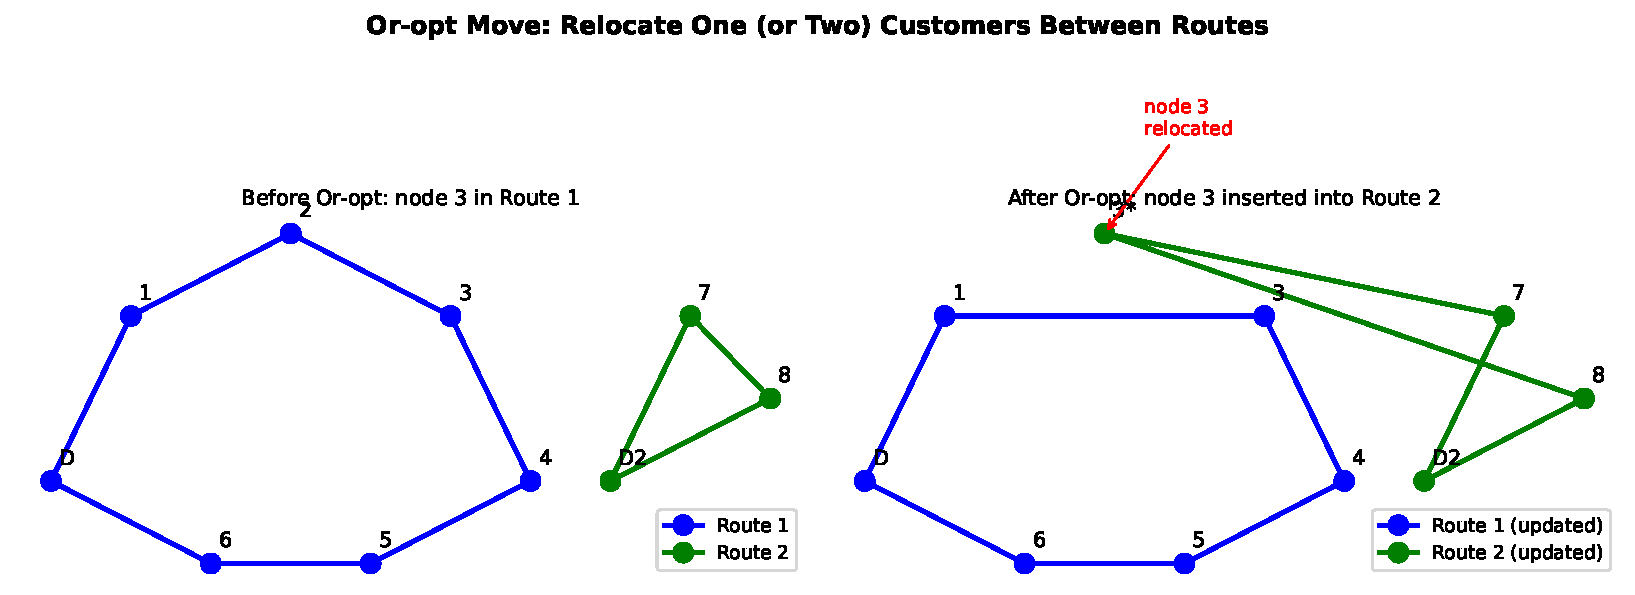
\includegraphics[width=0.7\textwidth]{or_opt.pdf}
  \end{center}

  \framebreak

  \begin{exampleblock}{Worked Example: Or-opt-1}
    Route 1: D$\to$1$\to$2$\to$3$\to$D with loads $(3,3,4)$, total
    load $=10=Q$.  Route 2: D$\to$4$\to$5$\to$D with loads $(2,2)$,
    total load $=4$.  Consider relocating customer 3 (load 4) to
    Route 2: new load of Route 2 $= 4+4=8 \le Q=10$.  The new
    routes are D$\to$1$\to$2$\to$D and D$\to$4$\to$3$\to$5$\to$D.
    If $d(2,3)+d(3,D)-d(2,D) > d(4,3)+d(3,5)-d(4,5)$ (removal saving
    exceeds insertion cost), the move reduces total distance.
  \end{exampleblock}

  \begin{alertblock}{Key Insight}
    Or-opt-1 is particularly effective for VRP because it can transfer
    customers between routes, reducing the total number of vehicles used
    and balancing route loads.  The Or-opt neighbourhood is strictly
    contained in the 3-opt neighbourhood.  In practice, combining 2-opt
    and Or-opt-1 within a single local-search procedure gives
    significantly better results than either operator alone.
  \end{alertblock}

\end{frame}

% ══════════════════════════════════════════════════════════════════════════════
\section{Metaheuristics}
% ══════════════════════════════════════════════════════════════════════════════

\begin{frame}[allowframebreaks]{Metaheuristics: Escaping Local Optima}

  Classical local search terminates at a local optimum — a solution that
  no single move improves — but this local optimum may be far from the
  global optimum.  \textbf{Metaheuristics} are higher-level strategies that
  guide local search to escape local optima and explore the solution space
  more broadly.

  \begin{block}{Three Paradigms for Escaping Local Optima}
    \begin{enumerate}
      \item \textbf{Memory-based} (Tabu Search): Forbid recently used moves
            to prevent cycling and force exploration of new regions.
      \item \textbf{Probabilistic acceptance} (Simulated Annealing): Accept
            worsening moves with a probability that decreases over time.
      \item \textbf{Population-based} (Genetic Algorithms, ACO): Maintain
            a set of solutions and combine them to generate new ones.
    \end{enumerate}
  \end{block}

  Since the publication of the first edition of the VRP book (2002),
  metaheuristics have become the dominant algorithmic paradigm for
  the VRP, with modern implementations consistently delivering solutions
  within \textbf{0.1--0.5\%} of the best known values on standard
  benchmarks.

\end{frame}

% ─── Tabu Search ─────────────────────────────────────────────────────────────
\begin{frame}[allowframebreaks]{Tabu Search}

  The word \emph{tabu} (also spelled \emph{taboo}) means ``forbidden.''
  Tabu Search (Glover, 1986) maintains a \textbf{tabu list} — a short-term
  memory of recently applied moves.  At each iteration, the algorithm
  selects the best non-tabu move, even if it worsens the objective.
  This prevents cycling back to recently visited solutions and forces
  the search into unexplored parts of the solution space.

  \begin{block}{Tabu Search Framework}
    \textbf{Given:} initial solution $s$, tabu list $\mathcal{T} = \emptyset$,
    best known solution $s^* = s$, tabu tenure $\tau$.
    \begin{enumerate}
      \item Generate all neighbours $\mathcal{N}(s)$.
      \item Select the best $s' \in \mathcal{N}(s)$ such that the move
            $m(s \to s')$ is \emph{not} in $\mathcal{T}$ \textbf{or}
            $s'$ satisfies the \textbf{aspiration criterion}
            (i.e., $c(s') < c(s^*)$, meaning it is better than the
            best known solution regardless of tabu status).
      \item Set $s \leftarrow s'$; add $m$ to $\mathcal{T}$; if
            $|\mathcal{T}| > \tau$, remove the oldest entry.
      \item If $c(s) < c(s^*)$, update $s^* \leftarrow s$.
      \item Repeat until stopping criterion (time limit or iteration
            limit) is reached.
    \end{enumerate}
    \textbf{Return} $s^*$.
  \end{block}

  \begin{center}
    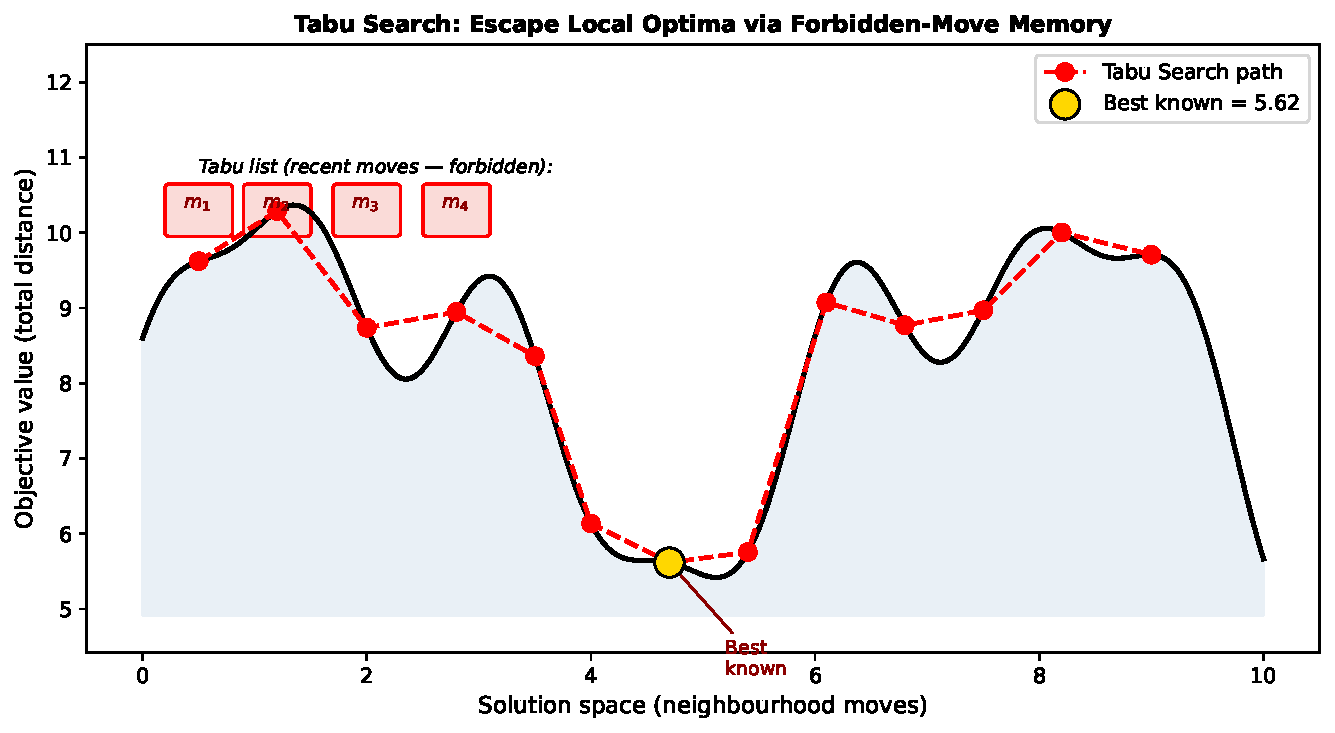
\includegraphics[width=0.65\textwidth]{tabu_search.pdf}
  \end{center}

  \framebreak

  \begin{block}{Tabu Search for VRP: Key Design Choices}
    \begin{itemize}
      \item \textbf{Move type:} Or-opt relocations (remove customer $v$
            from route $R_1$, insert into route $R_2$) are the most
            common tabu move for VRP.
      \item \textbf{What is made tabu:} The pair $(v, R_1)$ is placed on
            the tabu list, preventing customer $v$ from returning to
            route $R_1$ for the next $\tau$ iterations.
      \item \textbf{Tabu tenure $\tau$:} The length of the tabu list.
            Typical values for VRP are $\tau \in [5, 20]$.  Too short
            a tenure leads to cycling; too long a tenure over-restricts
            the search.
      \item \textbf{Penalty for infeasibility:} Many VRP Tabu Search
            implementations allow temporarily infeasible solutions
            (exceeding capacity) and penalise them with a term
            $\lambda \cdot \max(0, \text{excess load})$, where $\lambda$
            is a self-adjusting penalty coefficient.  This enlarges the
            effective search space.
    \end{itemize}
  \end{block}

  Among the most successful Tabu Search algorithms for the VRP are those
  of Taillard (1993), Rochat and Taillard (1995), Gendreau, Hertz, and
  Laporte (1994) (GENIUS/TABUROUTE), and the implementations of Cordeau,
  Gendreau, and Laporte (1997) for the VRPTW.

  \begin{alertblock}{Key Insight}
    The aspiration criterion is critical: it allows the algorithm to
    accept a tabu move when doing so would produce a new best solution.
    Without it, the tabu list might prevent the discovery of the global
    optimum.
  \end{alertblock}

\end{frame}

% ─── Simulated Annealing ──────────────────────────────────────────────────────
\begin{frame}[allowframebreaks]{Simulated Annealing}

  The analogy behind Simulated Annealing (SA) comes from metallurgy:
  when a metal is heated to a high temperature and then slowly cooled
  (\emph{annealed}), its atoms settle into a low-energy crystalline
  structure.  Kirkpatrick, Gelatt, and Vecchi (1983) observed that
  this physical process can be mimicked in combinatorial optimisation
  to escape local optima.

  \begin{block}{Simulated Annealing Algorithm}
    \textbf{Given:} initial solution $s$, initial temperature $T_0$,
    cooling rate $\alpha \in (0,1)$, stopping temperature $T_{\min}$.
    \begin{enumerate}
      \item Set $T \leftarrow T_0$, $s^* \leftarrow s$.
      \item \textbf{While} $T > T_{\min}$:
        \begin{enumerate}
          \item[(a)] Sample a random neighbour $s' \in \mathcal{N}(s)$.
          \item[(b)] Compute $\Delta C = c(s') - c(s)$.
          \item[(c)] If $\Delta C < 0$: accept $s \leftarrow s'$
                (improvement always accepted).
          \item[(d)] If $\Delta C \ge 0$: accept $s \leftarrow s'$
                with probability
                $p = \exp(-\Delta C / T)$.
          \item[(e)] If $c(s) < c(s^*)$: update $s^* \leftarrow s$.
        \end{enumerate}
      \item Apply cooling: $T \leftarrow \alpha \cdot T$.
      \item \textbf{Return} $s^*$.
    \end{enumerate}
  \end{block}

  \begin{center}
    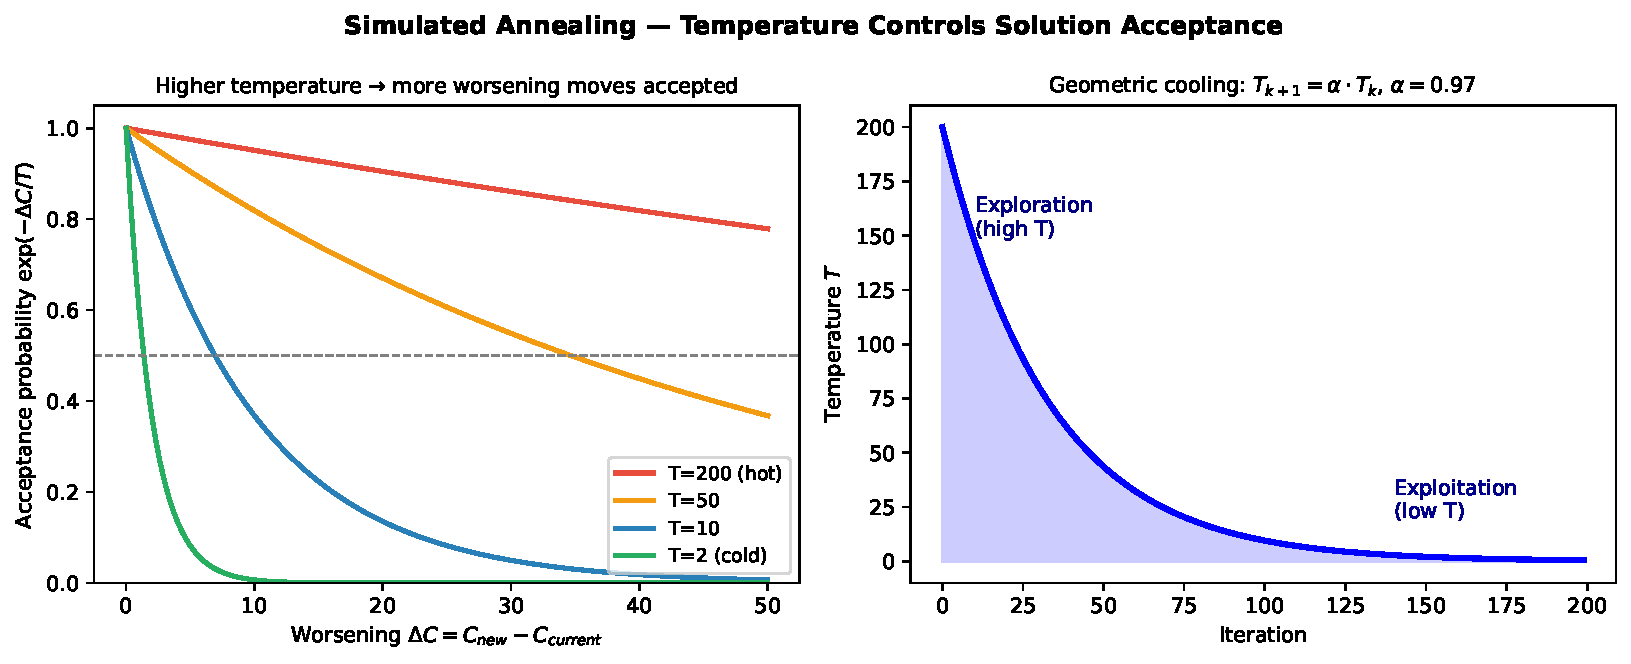
\includegraphics[width=0.78\textwidth]{simulated_annealing.pdf}
  \end{center}

  \framebreak

  \begin{block}{Interpreting the Acceptance Probability}
    The acceptance probability $p = \exp(-\Delta C / T)$ has two important
    properties.  First, it is always between 0 and 1, so the algorithm
    may accept worsening moves but never with certainty.  Second, as the
    temperature $T$ decreases toward zero, $p \to 0$ for any $\Delta C > 0$,
    meaning the algorithm becomes increasingly deterministic and converges
    toward a pure local search.  The geometric cooling schedule
    $T_k = \alpha^k T_0$ is the most common in practice.
  \end{block}

  \begin{exampleblock}{Numerical Example of Acceptance}
    Suppose the current solution has cost $c(s) = 1000$ and a randomly
    sampled neighbour has cost $c(s') = 1020$, so $\Delta C = 20$.
    At temperature $T = 50$: acceptance probability $= \exp(-20/50)
    \approx 0.67$ (67\% chance of accepting the worse solution).
    At $T = 5$: probability $= \exp(-20/5) \approx 0.018$ (less than 2\%).
    This shows how early in the run (high $T$) the algorithm explores
    broadly, while late in the run (low $T$) it exploits a good region.
  \end{exampleblock}

  \begin{alertblock}{Key Insight}
    SA's strength is its theoretical guarantee of convergence to the
    global optimum under a sufficiently slow cooling schedule
    (\emph{logarithmic cooling}), although in practice geometric cooling
    is used for computational efficiency.  SA applied to the VRP with
    Or-opt moves was popularised by Osman (1993) and Thompson and
    Psaraftis (1993).
  \end{alertblock}

\end{frame}

% ─── Genetic Algorithms ───────────────────────────────────────────────────────
\begin{frame}[allowframebreaks]{Genetic Algorithms}

  Genetic Algorithms (GAs), introduced by Holland (1975) and applied to
  combinatorial optimisation by Goldberg (1989), are population-based
  metaheuristics inspired by biological evolution.  The key idea is to
  maintain a \textbf{population} of solutions (``individuals'') and
  iteratively combine pairs of solutions via \textbf{crossover} and
  \textbf{mutation} to produce new solutions (``offspring'').  Good
  solutions survive preferentially to the next generation through
  \textbf{selection}.

  \begin{block}{Genetic Algorithm for VRP}
    \begin{enumerate}
      \item \textbf{Initialise} a population of $P$ feasible VRP
            solutions (using constructive heuristics or random construction).
      \item \textbf{Evaluate} each solution's fitness $= 1 / c(s)$.
      \item \textbf{While} stopping criterion not met:
        \begin{enumerate}
          \item[(a)] \textbf{Selection:} Choose two parents $s_1, s_2$
                by tournament or roulette-wheel selection.
          \item[(b)] \textbf{Crossover:} Apply an order-preserving
                crossover operator (e.g., OX or PMX) to produce child $s'$.
          \item[(c)] \textbf{Repair:} Fix infeasibilities (duplicate
                customers, capacity violations).
          \item[(d)] \textbf{Mutation:} With probability $p_m$, apply a
                random local move to $s'$.
          \item[(e)] \textbf{Local search:} Optionally improve $s'$
                with 2-opt or Or-opt (creating a ``memetic algorithm'').
          \item[(f)] \textbf{Replacement:} Insert $s'$ into the
                population, removing the worst individual.
        \end{enumerate}
      \item \textbf{Return} best solution found.
    \end{enumerate}
  \end{block}

  \begin{center}
    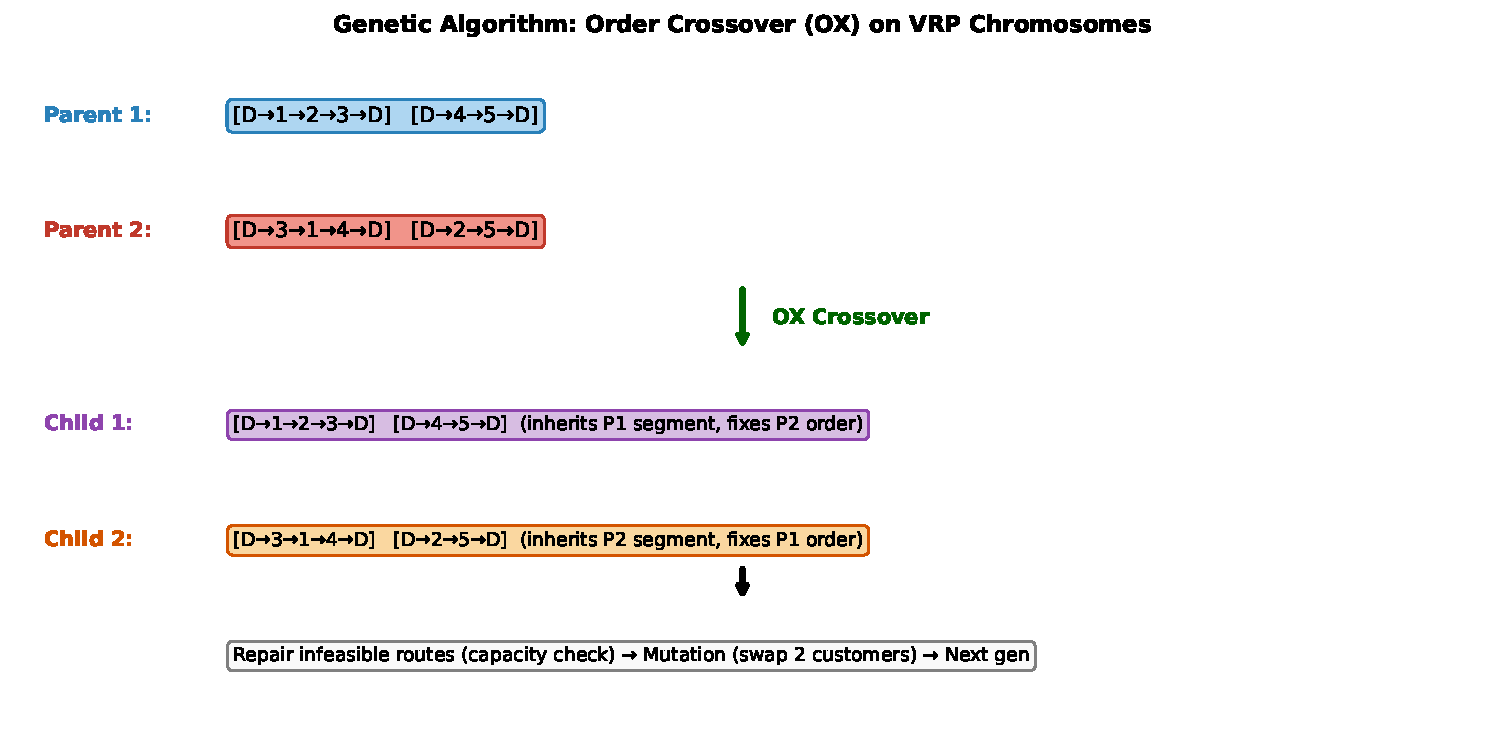
\includegraphics[width=0.72\textwidth]{genetic_algorithm.pdf}
  \end{center}

  \framebreak

  \begin{block}{VRP Crossover: The Challenge of Feasibility}
    Unlike binary or integer problems, VRP solutions are permutations of
    customers partitioned into routes.  Standard crossover operators
    can produce offspring with duplicate customers (a customer visited
    by two routes) or missing customers.  The \textbf{Order Crossover}
    (OX) operator handles this by inheriting one parent's route
    structure for a subset of customers and filling in the rest in the
    order they appear in the second parent.  Capacity constraints must
    then be re-checked and routes split or merged to restore feasibility.
  \end{block}

  Among the most successful GAs for the VRP are the Hybrid Genetic
  Algorithm (HGA) of Vidal et al.\ (2012, 2014), which combines
  an advanced OX-based crossover with intensive local search (2-opt,
  Or-opt, 3-opt) and a diversity management mechanism that prevents
  premature convergence.  The HGA has achieved top performance on
  virtually all standard VRP benchmarks.

  \begin{alertblock}{Key Insight}
    The term \textbf{memetic algorithm} describes a GA that includes
    local search as a post-crossover improvement step.  For the VRP,
    the local-search component is essential: without it, GAs typically
    produce solutions of similar quality to constructive heuristics.
    The power of GAs lies in their ability to combine \emph{building
    blocks} from different good solutions via crossover.
  \end{alertblock}

\end{frame}

% ─── Ant Colony Optimisation ──────────────────────────────────────────────────
\begin{frame}[allowframebreaks]{Ant Colony Optimisation (ACO)}

  Ant Colony Optimisation was introduced by Dorigo, Maniezzo, and Colorni
  (1991) inspired by the foraging behaviour of real ants.  Real ants
  deposit \textbf{pheromone} on paths they travel, and other ants
  preferentially follow high-pheromone paths.  Over time, shorter paths
  accumulate more pheromone (because ants return faster and reinforce
  them more) and longer paths evaporate their pheromone.  ACO mimics
  this collective behaviour to construct good solutions.

  \begin{block}{ACO Algorithm for VRP}
    \textbf{Initialise:} pheromone $\tau(i,j) = \tau_0$ for all edges;
    heuristic desirability $\eta(i,j) = 1/d_{ij}$.
    \begin{enumerate}
      \item \textbf{For} each of $m$ ants:
        \begin{enumerate}
          \item[(a)] Construct a complete VRP solution by building
                routes probabilistically: at position $i$, ant $k$
                chooses the next customer $j$ with probability
                \[
                  p_{ij}^k = \frac{[\tau(i,j)]^\alpha \cdot [\eta(i,j)]^\beta}
                    {\sum_{\ell \in \mathcal{F}} [\tau(i,\ell)]^\alpha
                    \cdot [\eta(i,\ell)]^\beta}
                \]
                where $\mathcal{F}$ is the set of feasible next customers,
                $\alpha$ controls pheromone influence, and $\beta$ controls
                distance influence.
          \item[(b)] Optionally improve each ant's solution with local
                search.
        \end{enumerate}
      \item \textbf{Pheromone update:}
        \begin{itemize}
          \item Evaporate: $\tau(i,j) \leftarrow (1-\rho)\,\tau(i,j)$
                for all $(i,j)$.
          \item Deposit: for each ant $k$ that used edge $(i,j)$,
                $\tau(i,j) \leftarrow \tau(i,j) + \Delta\tau^k(i,j)$
                where $\Delta\tau^k = Q_{\text{ACO}} / c(s^k)$.
        \end{itemize}
      \item Repeat for $T_{\max}$ iterations.  \textbf{Return} best solution.
    \end{enumerate}
  \end{block}

  \begin{center}
    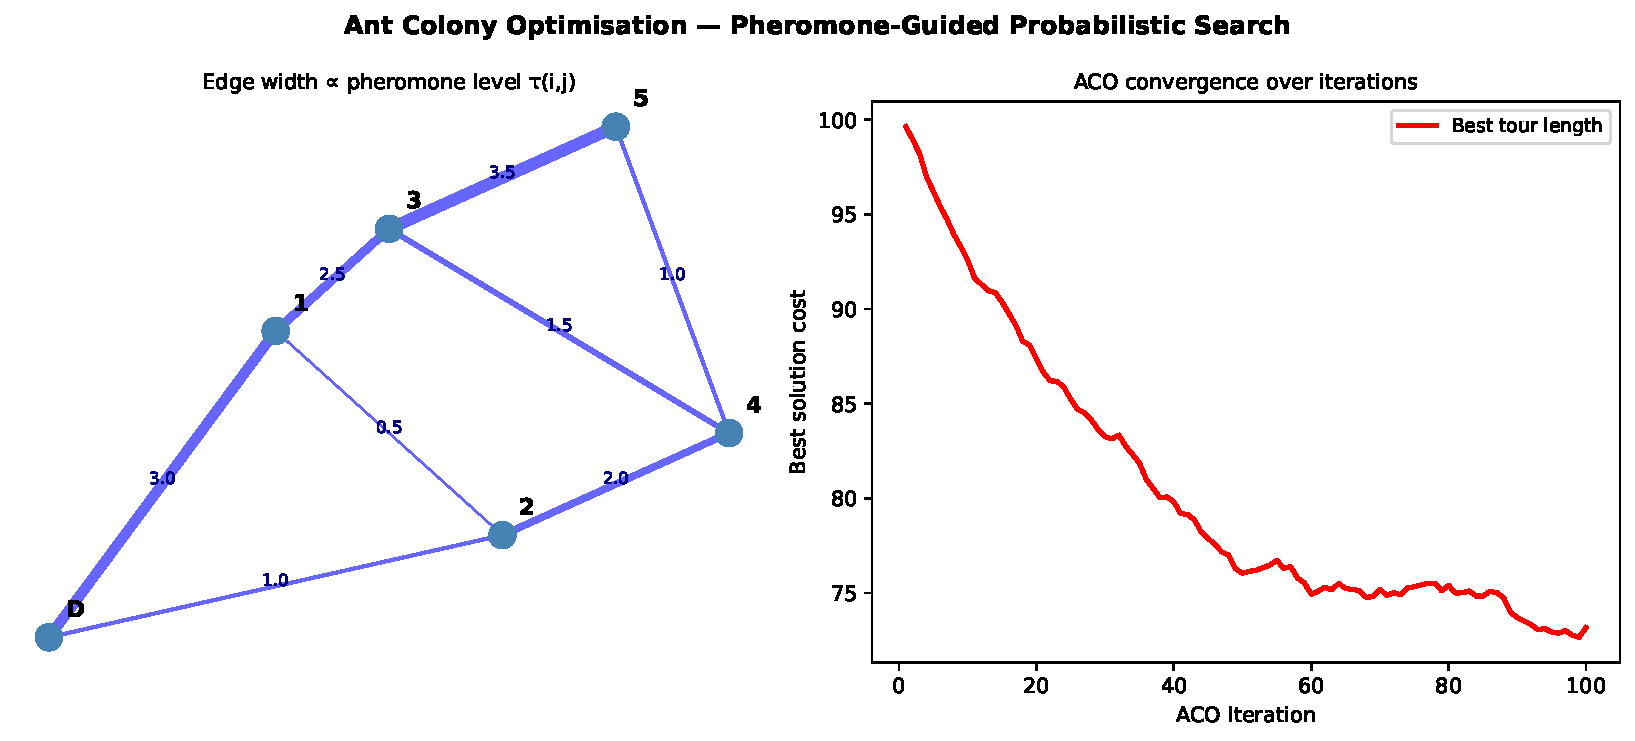
\includegraphics[width=0.65\textwidth]{aco.pdf}
  \end{center}

  \framebreak

  \begin{exampleblock}{Interpreting the Probability Formula}
    Consider an ant at customer $i$ choosing between customers $j=3$
    (distance 2, pheromone 4) and $k=7$ (distance 1, pheromone 1).
    With $\alpha=1, \beta=2$:
    \begin{align*}
      p_{i3} &\propto \tau(i,3)^1 \cdot \eta(i,3)^2 = 4 \cdot (1/2)^2 = 1.0 \\
      p_{i7} &\propto \tau(i,7)^1 \cdot \eta(i,7)^2 = 1 \cdot (1/1)^2 = 1.0
    \end{align*}
    Both customers are equally likely to be chosen despite customer 7
    being twice as close, because customer 3 has four times more
    pheromone.  This illustrates the tension between exploiting good
    historical routes (pheromone) and exploiting proximity (distance).
  \end{exampleblock}

  Among the most successful ACO implementations for VRP are those of
  Reimann, Doerner, and Hartl (2004) and the approach of Bell and
  McMullen (2004).

  \begin{alertblock}{Key Insight}
    ACO is naturally suited to problems where the quality of a solution
    depends on pairs of entities (edges, arcs), because pheromones are
    assigned to edges.  The combination of pheromone guidance and
    local search is key to ACO performance: without local search, ACO
    tends to produce mediocre solutions.
  \end{alertblock}

\end{frame}

% ─── Large Neighbourhood Search ───────────────────────────────────────────────
\begin{frame}[allowframebreaks]{Large Neighbourhood Search (LNS)}

  Large Neighbourhood Search (LNS), introduced by Shaw (1998) for the
  VRP, is based on the principle that good solutions share structural
  features (routes, sub-sequences) with other good solutions.  Rather
  than making small local moves, LNS alternates between a
  \textbf{destroy} phase (removing a large portion of the current
  solution) and a \textbf{repair} phase (rebuilding the destroyed
  portion, ideally better than before).

  \begin{block}{LNS Algorithm}
    \begin{enumerate}
      \item \textbf{Initialise:} construct a feasible solution $s$;
            set $s^* \leftarrow s$.
      \item \textbf{Repeat} until stopping criterion:
        \begin{enumerate}
          \item[(a)] \textbf{Destroy:} Remove $q$ customers from $s$
                using a destroy operator (random removal, worst removal,
                or Shaw's related removal).  Obtain partial solution
                $s_{\text{partial}}$.
          \item[(b)] \textbf{Repair:} Re-insert all removed customers
                into $s_{\text{partial}}$ using a greedy or
                regret-based insertion heuristic.  Obtain $s'$.
          \item[(c)] \textbf{Accept:} If $c(s') < c(s)$, set
                $s \leftarrow s'$.  (Simulated Annealing acceptance
                can also be used.)
          \item[(d)] If $c(s') < c(s^*)$, set $s^* \leftarrow s'$.
        \end{enumerate}
      \item \textbf{Return} $s^*$.
    \end{enumerate}
  \end{block}

  \begin{center}
    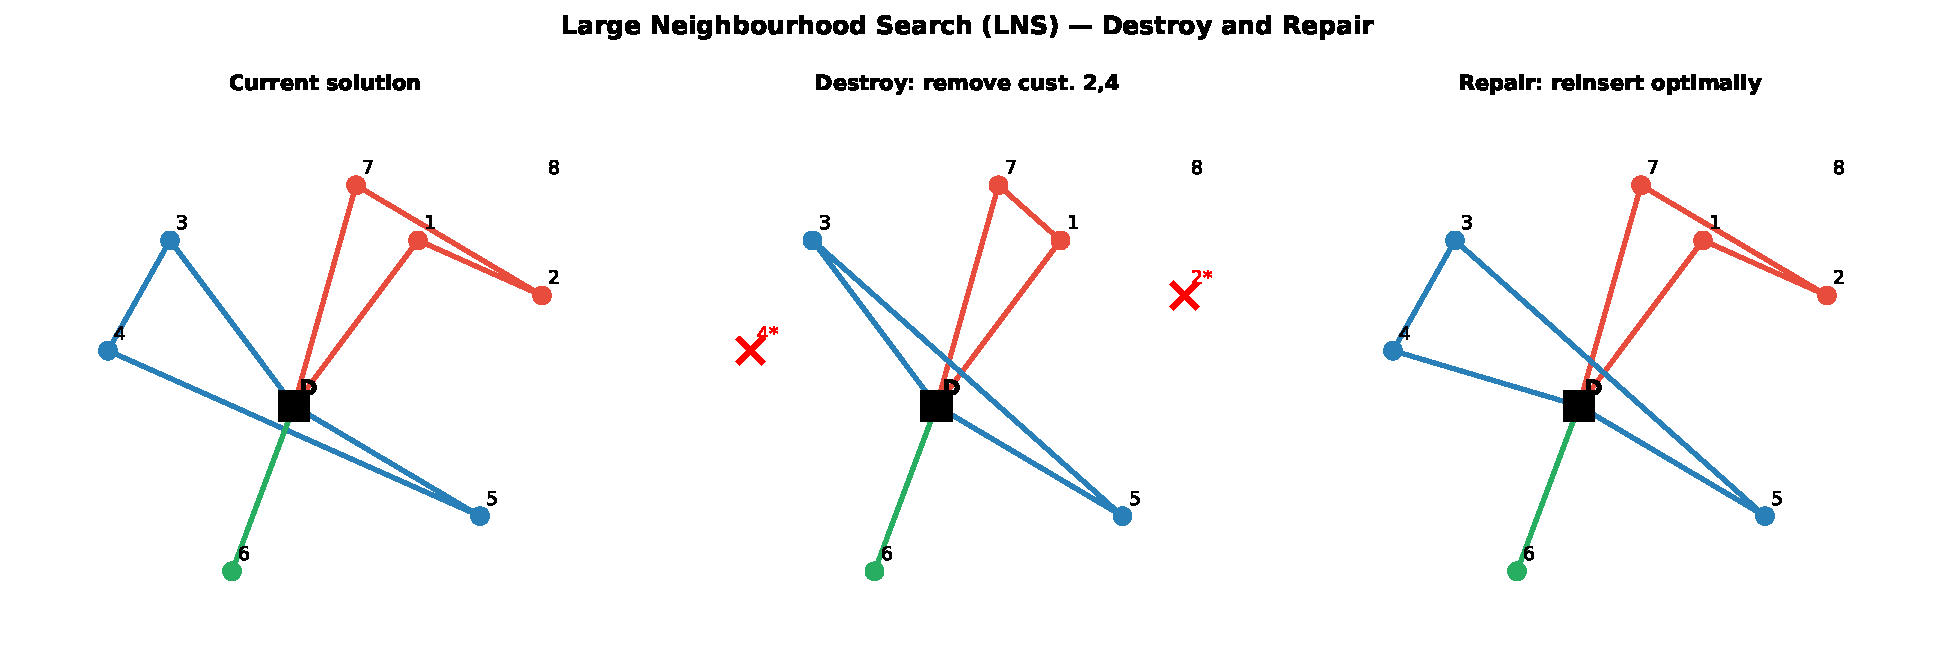
\includegraphics[width=0.82\textwidth]{lns.pdf}
  \end{center}

  \framebreak

  \begin{block}{Shaw's Related Removal Operator}
    Shaw's destroy operator removes customers that are \emph{related}
    to a seed customer $u$: a customer $v$ is related to $u$ if it is
    geographically close, has a similar time window, or is on the same
    route.  The relatedness of customers $u$ and $v$ is measured as:
    \[
      \text{rel}(u, v) = \phi \cdot d_{uv}
                       + \chi \cdot |T_u - T_v|
                       + \psi \cdot (1 - \mathbf{1}[\text{same route}])
    \]
    where $\phi, \chi, \psi$ are weighting parameters.  Removing related
    customers creates a ``hole'' in the solution that can be repaired in
    multiple ways, enabling large improvements.
  \end{block}

  \begin{block}{Adaptive LNS (ALNS) — Pisinger and Ropke (2007)}
    The Adaptive LNS extends LNS by maintaining a \emph{bank} of destroy
    and repair operators and selecting them probabilistically, with
    probabilities updated based on past performance (operators that
    have recently improved the solution are chosen more often).  ALNS
    is one of the most versatile and successful metaheuristics for VRP,
    with implementations achieving top results on the CVRP, VRPTW,
    PDPTW, and many other variants.
  \end{block}

  \begin{alertblock}{Key Insight}
    LNS operates on a much larger neighbourhood than classical local
    search: removing and reinserting $q$ customers from $n$ total
    creates a neighbourhood of size $\binom{n}{q}$, which is exponential
    in $q$.  Yet each iteration remains computationally tractable because
    the repair phase uses efficient insertion heuristics rather than
    exhaustive enumeration.
  \end{alertblock}

\end{frame}

% ─── Python: Savings + 2-opt ──────────────────────────────────────────────────
\begin{frame}[fragile]{Python Implementation: Clarke-Wright Savings Algorithm}
\begin{lstlisting}
import numpy as np

def clarke_wright_savings(coords, demands, capacity):
    """
    Clarke-Wright parallel savings algorithm for CVRP.
    coords  : list of (x,y); index 0 is the depot
    demands : list of demands; demands[0] = 0 (depot)
    capacity: vehicle capacity Q
    Returns a list of routes (each route is a list of customer indices).
    """
    n = len(coords) - 1  # number of customers (1..n)
    # Euclidean distance matrix
    def dist(i, j):
        return np.hypot(coords[i][0]-coords[j][0], coords[i][1]-coords[j][1])

    # Step 1: compute all savings s(i,j) for i,j in 1..n
    savings = []
    for i in range(1, n+1):
        for j in range(i+1, n+1):
            s = dist(0, i) + dist(0, j) - dist(i, j)
            savings.append((s, i, j))
    savings.sort(reverse=True)  # sort descending

    # Step 2: initialise n single-customer routes
    routes  = {i: [i] for i in range(1, n+1)}  # route_id -> [customers]
    in_route = {i: i for i in range(1, n+1)}    # customer -> route_id
    loads   = {i: demands[i] for i in range(1, n+1)}
    # track endpoints: start/end customers touching the depot
    start = {i: i for i in range(1, n+1)}  # first customer in route
    end   = {i: i for i in range(1, n+1)}  # last customer in route

    # Step 3: greedily merge routes
    for s, i, j in savings:
        ri, rj = in_route.get(i), in_route.get(j)
        if ri is None or rj is None or ri == rj:
            continue
        # i must be the LAST customer of route ri (adjacent to depot)
        # j must be the FIRST customer of route rj
        if end[ri] == i and start[rj] == j:
            if loads[ri] + loads[rj] <= capacity:
                # Merge: append rj after ri
                routes[ri].extend(routes[rj])
                new_load = loads[ri] + loads[rj]
                new_end  = end[rj]
                for c in routes[rj]:
                    in_route[c] = ri
                loads[ri] = new_load
                end[ri]   = new_end
                start[ri] = start[ri]
                del routes[rj], loads[rj], start[rj], end[rj]

    return list(routes.values())


# Example usage
if __name__ == '__main__':
    coords  = [(0,0),(2,3),(4,2),(6,3),(5,1),(1,4)]  # depot + 5 customers
    demands = [0, 2, 3, 2, 3, 2]
    Q = 7
    routes = clarke_wright_savings(coords, demands, Q)
    for r in routes:
        print('Route:', [0] + r + [0])
\end{lstlisting}
\end{frame}

\begin{frame}[fragile]{Python Implementation: 2-opt Local Search}
\begin{lstlisting}
import numpy as np

def two_opt(route, dist_matrix):
    """
    Apply 2-opt improvement to a single TSP route.
    route      : list of node indices (includes depot at start/end)
    dist_matrix: 2D numpy array of distances
    Returns improved route.
    """
    best = route[:]
    improved = True
    while improved:
        improved = False
        n = len(best)
        for i in range(1, n - 2):          # i is first edge start
            for j in range(i + 1, n - 1):  # j is second edge start
                # Current edges: (best[i-1], best[i]) and (best[j], best[j+1])
                d_before = (dist_matrix[best[i-1], best[i]]
                          + dist_matrix[best[j],   best[j+1]])
                # After reversing segment best[i..j]:
                d_after  = (dist_matrix[best[i-1], best[j]]
                          + dist_matrix[best[i],   best[j+1]])
                if d_after < d_before - 1e-10:
                    best[i:j+1] = best[i:j+1][::-1]  # reverse segment
                    improved = True
    return best


def two_opt_vrp(routes, coords):
    """Apply 2-opt to each route in a VRP solution."""
    n_nodes = len(coords)
    D = np.zeros((n_nodes, n_nodes))
    for i in range(n_nodes):
        for j in range(n_nodes):
            D[i, j] = np.hypot(coords[i][0]-coords[j][0],
                               coords[i][1]-coords[j][1])
    improved_routes = []
    for route in routes:
        full = [0] + route + [0]       # add depot at both ends
        improved = two_opt(full, D)
        improved_routes.append(improved[1:-1])  # strip depot
    return improved_routes


# Example usage
if __name__ == '__main__':
    coords = [(0,0),(1,1),(3,2),(2,4),(5,1),(4,3)]
    route  = [1, 3, 5, 2, 4]   # customer visit order
    routes = two_opt_vrp([route], coords)
    print('Improved route:', routes[0])
\end{lstlisting}
\end{frame}

\begin{frame}[fragile]{Python Implementation: Or-opt-1 (Customer Relocation)}
\begin{lstlisting}
import numpy as np
from itertools import product

def or_opt1(routes, coords, demands, capacity):
    """
    Or-opt-1: try relocating every customer to every other position
    in any route.  Apply the best improving move and repeat.
    """
    n_nodes = len(coords)
    D = np.zeros((n_nodes, n_nodes))
    for i in range(n_nodes):
        for j in range(n_nodes):
            D[i, j] = np.hypot(coords[i][0]-coords[j][0],
                               coords[i][1]-coords[j][1])

    def route_load(r):
        return sum(demands[c] for c in r)

    def route_cost(r):
        full = [0] + r + [0]
        return sum(D[full[k], full[k+1]] for k in range(len(full)-1))

    improved = True
    while improved:
        improved = False
        best_gain, best_move = 0, None
        for ri in range(len(routes)):
            for pos_v in range(len(routes[ri])):
                v = routes[ri][pos_v]
                # removal gain: removing v from route ri
                r_before = [0] + routes[ri] + [0]
                pred = r_before[pos_v]      # node before v
                succ = r_before[pos_v + 2]  # node after v
                gain_remove = (D[pred, v] + D[v, succ] - D[pred, succ])
                for rj in range(len(routes)):
                    # check capacity if different route
                    if ri != rj and route_load(routes[rj]) + demands[v] > capacity:
                        continue
                    target = routes[rj] if ri != rj else (
                             routes[ri][:pos_v] + routes[ri][pos_v+1:])
                    for ins_pos in range(len(target) + 1):
                        a = 0 if ins_pos == 0 else target[ins_pos-1]
                        b = 0 if ins_pos == len(target) else target[ins_pos]
                        cost_insert = D[a, v] + D[v, b] - D[a, b]
                        gain = gain_remove - cost_insert
                        if gain > best_gain + 1e-10:
                            best_gain = gain
                            best_move = (ri, pos_v, rj, ins_pos)
        if best_move:
            ri, pos_v, rj, ins_pos = best_move
            v = routes[ri].pop(pos_v)
            if ri == rj and ins_pos > pos_v:
                ins_pos -= 1
            routes[rj].insert(ins_pos, v)
            improved = True
    return routes
\end{lstlisting}
\end{frame}

% ══════════════════════════════════════════════════════════════════════════════
\section{Hybridizations}
% ══════════════════════════════════════════════════════════════════════════════

\begin{frame}[allowframebreaks]{Hybridizations}

  A \textbf{hybridization} of metaheuristics combines ideas from
  two or more paradigms in order to benefit from the strengths of each.
  Population-based methods such as genetic algorithms are good at
  \emph{diversification} (exploring many different regions of the
  solution space) but slow at \emph{intensification} (refining a
  particular good solution).  Conversely, single-solution methods such
  as Tabu Search excel at intensification but may miss important regions
  of the solution space.

  \begin{block}{Main Hybridization Paradigms for VRP}
    \begin{enumerate}
      \item \textbf{Population-based search + local search (Memetic
            Algorithms):} The most successful approach.  Each individual
            in the population is locally optimised (using 2-opt, Or-opt,
            LK) before being evaluated.  Examples include the HGA of
            Vidal et al.\ (2012) and the EAX-based method of Nagata,
            Braysy, and Dullaert (2010).
      \item \textbf{Tabu Search + path relinking:} Rochat and Taillard
            (1995) maintain a pool of elite solutions.  When the TS is
            diversified, it ``path-relinks'' the current solution toward
            an elite solution, exploring the corridor of solutions between
            the two.
      \item \textbf{Scatter Search and GRASP:} Scatter search combines a
            reference set of diverse good solutions; GRASP (Greedy
            Randomised Adaptive Search Procedure) alternates between
            randomised constructive phases and local-search improvement
            phases.
    \end{enumerate}
  \end{block}

  \framebreak

  \begin{block}{Population-based Hybridization with Diversity Management}
    One of the key challenges in hybrid GA is premature convergence: if
    all individuals in the population become too similar, crossover stops
    producing novel offspring.  The HGA of Vidal et al.\ (2012) addresses
    this through an explicit \textbf{diversity control} mechanism:
    \begin{itemize}
      \item The population is split into a \emph{feasible} and an
            \emph{infeasible} sub-population (infeasible solutions violate
            capacity constraints but may lead to good feasible solutions
            after repair).
      \item A \textbf{biased fitness} measure combines solution quality
            (objective value) and a \textbf{diversity contribution}
            (measured as average Hamming distance to the closest
            neighbours in the population).
      \item Individuals with low diversity contribution are periodically
            removed (\emph{survivor selection}).
    \end{itemize}
    This mechanism ensures that the population remains diverse throughout
    the search, sustaining effective crossover and leading to high-quality
    solutions.
  \end{block}

  \begin{block}{Decomposition and Parallelism}
    For very large instances (thousands of customers), parallelisation is
    essential.  Several parallel strategies have been proposed:
    \begin{itemize}
      \item \textbf{Spatial decomposition:} Partition the service area
            into sub-regions (sectors, strips, or Voronoi cells) and
            solve each sub-region independently (Figure~\ref{fig:decomp}).
      \item \textbf{Independent runs with elite exchange:} Run $P$
            independent metaheuristic threads and periodically exchange
            elite solutions between threads.
      \item \textbf{Centralised neighbourhood evaluation:} Use parallel
            threads to evaluate the neighbourhood in parallel, reducing
            the time per iteration.
    \end{itemize}
  \end{block}

  \begin{figure}
    \centering
    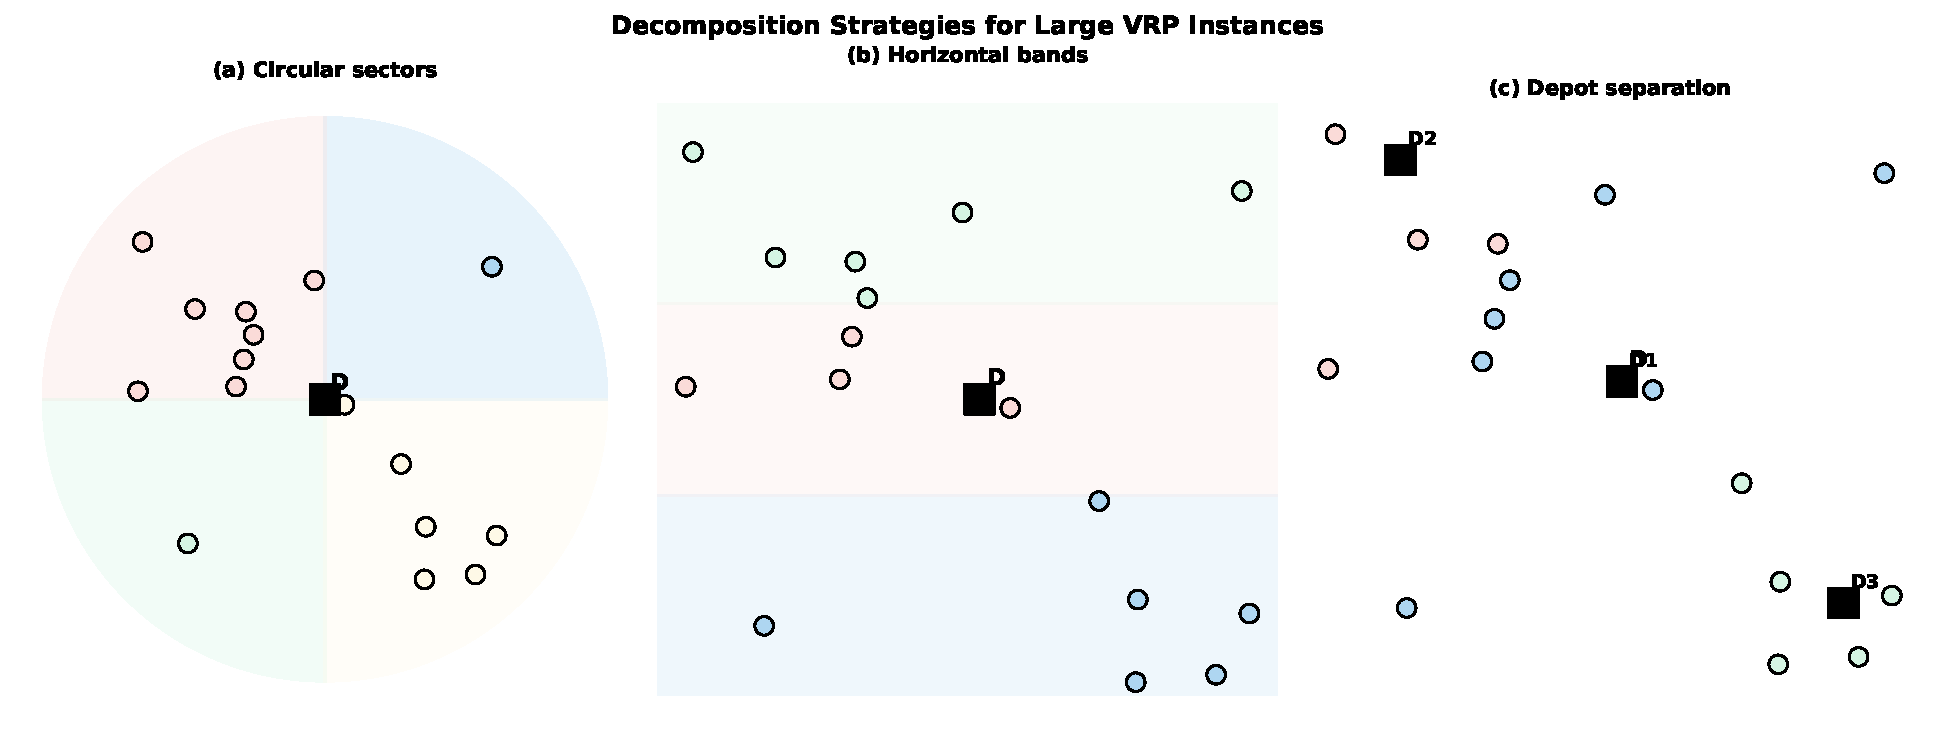
\includegraphics[width=0.85\textwidth]{decomposition.pdf}
    \caption{Three spatial decomposition strategies for large VRP instances:
      (a) circular sectors, (b) horizontal bands, (c) assignment to nearest
      depot.  Each colour denotes a separate sub-problem solved independently.}
    \label{fig:decomp}
  \end{figure}

\end{frame}

% ══════════════════════════════════════════════════════════════════════════════
\section{Unified Algorithms}
% ══════════════════════════════════════════════════════════════════════════════

\begin{frame}[allowframebreaks]{Unified Algorithms for Multi-Attribute VRP}

  The vast majority of real-world VRP instances involve additional
  constraints beyond simple capacity: time windows, heterogeneous
  fleets, multiple depots, split deliveries, backhauls, periodic
  scheduling, and so on.  Historically, a separate algorithm was
  designed for each variant.  \textbf{Unified algorithms} aim to solve
  a broad family of VRP variants with a \emph{single} algorithmic
  framework, adapting to specific attributes through parameterised
  constraint handling.

  \begin{block}{The Unified HGA of Vidal et al.\ (2014)}
    Vidal, Crainic, Gendreau, and Prins proposed a unified hybrid GA
    that handles a large class of multi-attribute VRPs.  The key
    design principles are:
    \begin{enumerate}
      \item \textbf{Giant-tour representation:} Solutions are encoded as
            a single sequence of all customers (a ``giant tour'').  The
            partition into routes is determined on the fly by an efficient
            \emph{split procedure}.
      \item \textbf{Split procedure:} Given a giant tour
            $(\pi_1, \pi_2, \ldots, \pi_n)$, the split algorithm solves
            a shortest-path problem on an auxiliary graph to find the
            optimal partition respecting capacity and other constraints.
            This runs in $O(n)$ time for CVRP and $O(n^2)$ for VRPTW.
      \item \textbf{Neighbourhood:} The GENIUS-style crossover and
            Or-opt / 2-opt / 3-opt local search operators are applied
            to the giant tour, with the split procedure converting
            the result back to routes at each evaluation.
    \end{enumerate}
  \end{block}

  \framebreak

  \begin{block}{Advantages of the Unified Approach}
    \begin{itemize}
      \item A \textbf{single codebase} handles CVRP, VRPTW, multi-depot
            VRP, periodic VRP, heterogeneous fleet VRP, and combinations
            thereof.
      \item The \textbf{split procedure} automatically enforces all
            feasibility constraints without requiring ad-hoc repair
            operators for each variant.
      \item \textbf{State-of-the-art performance} on all tested variants:
            the unified HGA achieved competitive or record-breaking
            solutions on CVRP, VRPTW, and several other benchmark
            families.
    \end{itemize}
  \end{block}

  \begin{block}{The Adaptive Attribute Selection Paradigm}
    Vidal et al.\ (2014) extend the unified framework further by
    introducing \textbf{adaptive attribute selection}: the algorithm
    automatically identifies which problem attributes (time windows,
    depot assignment, etc.) are ``active'' for a given instance and
    adjusts the split procedure and neighbourhood operators accordingly.
    This makes the framework applicable to instances with up to 10 or
    more simultaneous attributes.
  \end{block}

  \begin{alertblock}{Key Insight}
    The giant-tour representation with split decoding elegantly separates
    the combinatorial structure of route construction from the constraint
    evaluation.  It allows a single evolutionary operator (crossover)
    applied to the giant tour to implicitly explore an exponentially
    large space of feasible route partitions.
  \end{alertblock}

\end{frame}

% ══════════════════════════════════════════════════════════════════════════════
\section{Computational Comparison of Selected Metaheuristics}
% ══════════════════════════════════════════════════════════════════════════════

\begin{frame}[allowframebreaks]{Benchmark Instances and Comparison Methodology}

  The chapter presents a systematic computational comparison of
  metaheuristics on two standard benchmark sets.

  \begin{block}{Benchmark Data Sets}
    \begin{enumerate}
      \item \textbf{GWKC (Golden-Wasil-Kelly-Cheung)} instances: 20 large
            CVRP instances with $n \in \{240, 255, 280, 300, 320, 360, 396,
            400, 420, 440, 480, 483\}$ customers and various numbers of
            depots ($C$ = Christofides-type, $CD$ = combined).  These are
            the primary benchmark for comparing state-of-the-art
            metaheuristics.
      \item \textbf{CMT (Christofides-Mingozzi-Toth)} instances: 14
            classical instances with $n \in \{50, 75, 100, 150, 199\}$
            customers.  These smaller instances admit near-optimal
            solutions and serve as ground truth for exact methods.
    \end{enumerate}
  \end{block}

  \begin{block}{Performance Metrics}
    Two metrics are reported for each algorithm on each instance:
    \begin{itemize}
      \item \textbf{Solution value:} total travel distance of the best
            solution found.
      \item \textbf{Percentage gap:}
            $\displaystyle \text{gap} =
            \frac{c(s_{\text{alg}}) - c(s^*)}{c(s^*)} \times 100\%$,
            where $c(s^*)$ is the best known solution value across
            all algorithms and runs.
    \end{itemize}
    Running times are \textbf{normalised} to a reference machine speed
    using a benchmark program, making times comparable across different
    hardware.  The normalised time unit corresponds roughly to a 1~GHz
    processor running a standard sorting benchmark.
  \end{block}

  \framebreak

  \begin{block}{Algorithms in the Comparison}
    The following selected metaheuristics are compared (Table 4.2 of
    the book):
    \smallskip
    \begin{center}
    \small
    \begin{tabular}{lll}
      \toprule
      ID & Algorithm & Type \\
      \midrule
      CLM01 & Cordeau, Laporte, Mercier (2001) & Tabu Search \\
      TV03  & Tarantilis, Voratas (2003) & SA / TS hybrid \\
      RDH04 & Reimann, Doerner, Hartl (2004) & ACO \\
      T05   & Toth, Vigo --- granular TS (2003/2005) & Tabu Search \\
      MB07  & Mester, Br\"aysy (2007) & SA hybrid \\
      PRO7  & Prins (2004, 2009) & GA \\
      NB09  & Nagata, Br\"aysy (2009) & EAX GA \\
      P09   & Pisinger, Ropke (2010) & ALNS \\
      ZK10  & Zachariadis, Kiranoudis (2010) & TS \\
      GGW10 & Groer, Golden, Wasil (2010) & CLAM \\
      VCGLR12 & Vidal et al.\ (2012) & HGA \\
      GGW11 & Groer, Golden, Wasil (2011) & --- \\
      CGW11 & Chu, Gao, Wang (2011) & --- \\
      CM12  & Contardo, Martinelli (2012) & TS \\
      JCL12 & Jin, Chen, Lu (2012) & EA \\
      SUO13 & --- (2013) & HGA \\
      \bottomrule
    \end{tabular}
    \end{center}
  \end{block}

\end{frame}

\begin{frame}[allowframebreaks]{Computational Results: GWKC Instances}

  Tables 4.3--4.9 in the book report detailed results for all 20 GWKC
  instances.  We summarise the key findings here.

  \begin{block}{Selected Results from Table 4.7 (Part I)}
    \small
    \begin{center}
    \begin{tabular}{lccccc}
      \toprule
      \# & $n$ & Best known & CLM01 (\%) & TV03 (\%) & RDH04 (\%) \\
      \midrule
      1  & 240C  & 5623.47  & 5681.97 (1.04) & 5736.15 (2.00) & 5644.02 (0.37) \\
      4  & 480C  & 13592.88 & 13740.60 (1.09) & 14910.62 (9.69) & 13699.11 (0.78)\\
      5  & 200C  & 6460.98  & 6756.44 (4.57) & 6697.53 (3.66) & 6460.98 (0.00) \\
      8  & 440C  & 11635.34 & 11869.50 (2.01) & 12036.24 (3.45) & 11936.16 (2.59)\\
      11 & 399CD & 912.84   & 929.07 (1.78)  & 936.04 (2.54)  & 927.27 (1.58)  \\
      \midrule
      \multicolumn{3}{l}{Average gap} & 1.79\% & 2.06\% & 0.93\% \\
      \bottomrule
    \end{tabular}
    \end{center}
  \end{block}

  \begin{block}{Selected Results: Modern Methods (Tables 4.8--4.9)}
    \small
    \begin{center}
    \begin{tabular}{lcccc}
      \toprule
      ID & Avg.\ gap (\%) & Norm.\ time (s) & Type \\
      \midrule
      MB07 (best cfg) & 0.33 & 13005.5 & SA hybrid \\
      NB09 (best cfg) & 0.17 & 13005.5 & EAX GA \\
      P09  (best cfg) & 0.63 & 233.4   & ALNS \\
      GGW10 (best cfg)& 0.12 & 43.4    & CLAM \\
      VCGLR12 (best)  & 0.16 & 3387.5  & HGA \\
      GGW11 (best cfg)& 0.19 & 43.4    & --- \\
      CM12 (best cfg) & 0.56 & 18770.0 & TS \\
      JCL12 (best cfg)& 0.35 & 200978.4 & EA \\
      SUO13 (best cfg)& 0.40 & 39382.3  & HGA \\
      GGW11-A & 0.25 & 100000  & --- \\
      \bottomrule
    \end{tabular}
    \end{center}
  \end{block}

  \framebreak

  \begin{center}
    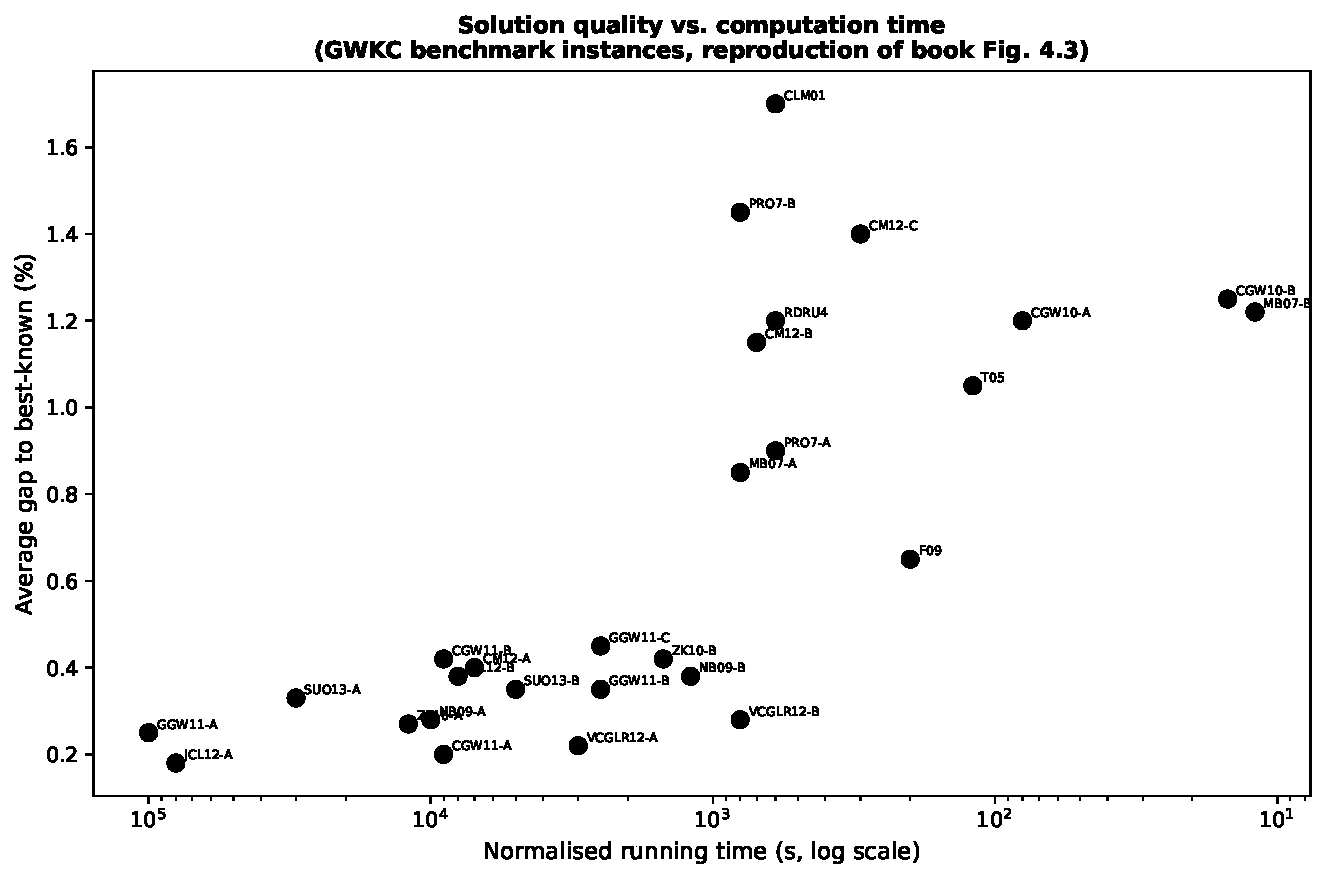
\includegraphics[width=0.85\textwidth]{quality_time_scatter.pdf}
  \end{center}

  The scatter plot above shows the trade-off between solution quality
  (average gap to best known, \%) and computation time (normalised
  seconds, log scale) for all algorithm configurations on the GWKC
  instances.  The ``Pareto frontier'' of non-dominated configurations
  runs from the bottom-left (fast and good) toward the bottom-right
  (slow but marginally better).

  \framebreak

  \begin{center}
    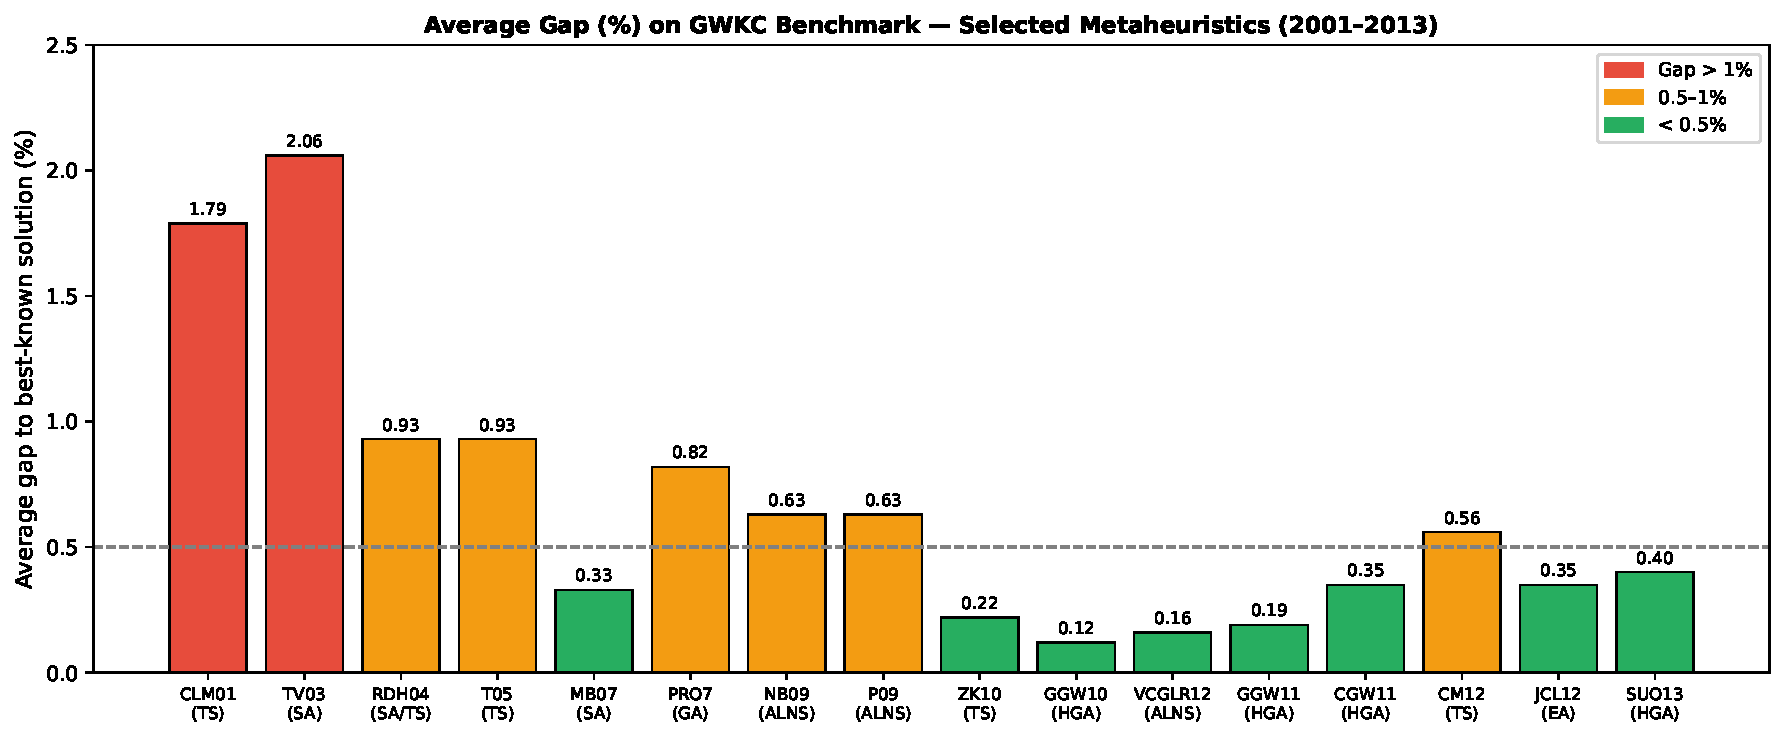
\includegraphics[width=0.92\textwidth]{gap_comparison.pdf}
  \end{center}

  The bar chart above illustrates the dramatic improvement in VRP
  heuristic quality over the period 2001--2013.  Early Tabu Search
  methods (CLM01) achieved gaps of $\sim$1.8\%, while modern Hybrid
  GAs and ALNS implementations (GGW10, VCGLR12, NB09) routinely
  achieve gaps of $\sim$0.1--0.2\% with comparable or shorter running
  times.

  \begin{alertblock}{Key Takeaway from the Computational Comparison}
    No single algorithm dominates all others on all instance types and
    time budgets.  For practitioners, the ALNS framework (Pisinger and
    Ropke) offers a good balance between solution quality and
    implementation complexity.  For research-level performance on the
    CVRP, Hybrid Genetic Algorithms (Vidal et al., Nagata et al.)
    currently represent the state of the art.
  \end{alertblock}

\end{frame}

\begin{frame}[allowframebreaks]{Other Measures of Quality and Robustness}

  Beyond average gap, the chapter discusses several additional evaluation
  dimensions that are important for a complete picture of algorithm
  performance.

  \begin{block}{Simplicity}
    A heuristic should be as simple as possible in its implementation,
    especially if it is to be applied in different problem settings.
    Algorithms that can be tuned with only a small number of parameters
    are preferred over those requiring elaborate configuration.  For
    example, the ALNS framework requires only the weight-update rule
    and a set of operators, while some Tabu Search implementations
    have dozens of interdependent parameters.
  \end{block}

  \begin{block}{Robustness Across Instance Types}
    An algorithm is \textbf{robust} if it achieves consistently good
    performance across all instances in a benchmark set, not just on
    average.  The standard deviation of the gap across instances is
    an important secondary metric.  Some algorithms achieve a low
    average gap but have high variance (performing excellently on
    some instances but poorly on others).
  \end{block}

  \begin{block}{Taking Advantage of Parallel Processing}
    Modern processors are massively parallel.  The chapter highlights
    that algorithms which run $k$ independent threads and report the
    best solution have an inherent advantage: running $k$ independent
    copies of a randomised algorithm for time $T/k$ each produces
    results that are statistically comparable to running a single copy
    for time $T$, but all $k$ copies can run simultaneously on a
    multi-core machine.
  \end{block}

\end{frame}

% ══════════════════════════════════════════════════════════════════════════════
\section{Conclusions and Future Research Directions}
% ══════════════════════════════════════════════════════════════════════════════

\begin{frame}[allowframebreaks]{Conclusions and Future Research Directions}

  Chapter 4 has presented a comprehensive survey of heuristics for
  the Vehicle Routing Problem, from the classical constructive methods
  of the 1960s--1970s to the sophisticated hybrid metaheuristics of
  the 2010s.  Several clear conclusions emerge from the computational
  evidence.

  \begin{block}{Main Conclusions}
    \begin{enumerate}
      \item \textbf{Metaheuristics dominate:} For any VRP instance large
            enough that exact methods are impractical, a well-implemented
            metaheuristic (Tabu Search, ALNS, or HGA) will find a solution
            within 0.5\% of the best known value.
      \item \textbf{Hybridization pays off:} Combining local search with
            population-based search (memetic algorithms) consistently
            outperforms either component in isolation.
      \item \textbf{Unified frameworks are the future:} As real-world
            VRP instances involve increasingly many simultaneous
            constraints, algorithms that can handle multiple attributes
            without redesign are highly valuable.
      \item \textbf{Benchmarks are essential:} The availability of
            standardised benchmark sets (GWKC, CMT, Solomon) and
            a common normalised time scale has enabled meaningful
            comparison across algorithms and hardware generations.
    \end{enumerate}
  \end{block}

  \framebreak

  \begin{block}{Future Research Directions}
    The chapter identifies several promising directions for future work:
    \begin{itemize}
      \item \textbf{Robustness vs.\ time:} Current top algorithms are
            often sensitive to parameter settings.  Developing
            parameter-free or self-calibrating methods would make
            them more accessible.
      \item \textbf{Very large-scale instances:} Instances with tens
            of thousands of customers are increasingly common in
            e-commerce logistics.  Decomposition methods and massively
            parallel algorithms are needed.
      \item \textbf{Dynamic and stochastic VRP:} Real-world routing
            involves uncertainty (stochastic demands, traffic
            disruptions, new customer requests arriving in real time).
            Metaheuristics need to be adapted to re-optimise solutions
            online with very short re-computation windows.
      \item \textbf{Machine learning integration:} Recent research
            explores using learned heuristics (neural combinatorial
            optimisation) either as standalone solvers or as
            components within classical metaheuristic frameworks
            (e.g., to learn good destroy/repair operators for LNS).
      \item \textbf{Multi-objective VRP:} Optimising simultaneously
            for cost, CO$_2$ emissions, and driver workload requires
            Pareto-front search methods adapted from multi-objective
            evolutionary computing.
    \end{itemize}
  \end{block}

  \begin{alertblock}{Overall Takeaway}
    The field of VRP heuristics is now sufficiently mature that near-optimal
    solutions to standard benchmark problems can be obtained routinely.
    The current research frontier has shifted to robustness across
    problem variants, scalability to very large instances, and
    integration with dynamic/stochastic settings and data-driven methods.
  \end{alertblock}

\end{frame}

% ══════════════════════════════════════════════════════════════════════════════
\section{Summary of Algorithms}
% ══════════════════════════════════════════════════════════════════════════════

\begin{frame}[allowframebreaks]{Algorithm Summary and Complexity Reference}

  The following table summarises the key heuristics covered in this
  chapter, their type, neighbourhood complexity, and typical solution
  quality on standard CVRP benchmarks.

  \begin{center}
  \small
  \begin{tabular}{>{\bfseries}lllcc}
    \toprule
    Algorithm & Type & Neighbourhood & Complexity & Typical gap \\
    \midrule
    Clarke-Wright   & Constructive  & ---           & $O(n^2 \log n)$ & 10--15\% \\
    Nearest Neighbour & Constructive & ---           & $O(n^2)$        & 20--25\% \\
    Sweep           & Constructive  & ---           & $O(n \log n)$   & 10--20\% \\
    2-opt           & Local search  & $O(n^2)$ per route & $O(n^2)$   & 5--10\%  \\
    3-opt           & Local search  & $O(n^3)$ per route & $O(n^3)$   & 3--7\%   \\
    Or-opt-1        & Local search  & $O(n^2)$      & $O(n^2)$        & 5--8\%   \\
    Lin-Kernighan   & Local search  & Variable      & $O(n^{2.5})$    & 1--3\%   \\
    Tabu Search     & Metaheuristic & $O(n^2)$ per iter & ---          & 0.5--2\% \\
    Sim.\ Annealing & Metaheuristic & $O(n)$ per iter   & ---          & 0.5--2\% \\
    Genetic Alg.    & Metaheuristic & Population-based  & ---          & 0.3--1\% \\
    ACO             & Metaheuristic & Population-based  & ---          & 0.5--1\% \\
    LNS / ALNS      & Metaheuristic & $O\!\binom{n}{q}$ & ---         & 0.2--0.5\% \\
    Hybrid GA (HGA) & Hybrid        & Population+LS     & ---          & 0.1--0.3\% \\
    \bottomrule
  \end{tabular}
  \end{center}

  \medskip
  Note: ``typical gap'' refers to the gap from the best known solution
  on CVRP benchmark instances (GWKC or CMT), and reflects the algorithm
  applied in isolation with standard parameter settings.  Hybrid
  implementations and careful parameter tuning generally achieve lower
  gaps than those shown here.

\end{frame}

% ══════════════════════════════════════════════════════════════════════════════
\section{Bibliography}
% ══════════════════════════════════════════════════════════════════════════════

\begin{frame}[allowframebreaks]{Key References}

  \begin{thebibliography}{99}
  \setbeamertemplate{bibliography item}[text]

  \bibitem{ClarkeWright1964}
    G.\ Clarke and J.\ W.\ Wright,
    \emph{Scheduling of vehicles from a central depot to a number of
      delivery points},
    Operations Research, 12 (1964), pp.\ 568--581.

  \bibitem{Gillett1974}
    B.\ E.\ Gillett and L.\ R.\ Miller,
    \emph{A heuristic algorithm for the vehicle-dispatch problem},
    Operations Research, 22 (1974), pp.\ 340--349.

  \bibitem{Lin1965}
    S.\ Lin,
    \emph{Computer solutions of the traveling salesman problem},
    Bell System Technical Journal, 44 (1965), pp.\ 2245--2269.

  \bibitem{LinKernighan1973}
    S.\ Lin and B.\ W.\ Kernighan,
    \emph{An effective heuristic algorithm for the traveling-salesman problem},
    Operations Research, 21 (1973), pp.\ 498--516.

  \bibitem{Or1976}
    I.\ Or,
    \emph{Traveling salesman-type combinatorial problems and their
      relation to the logistics of regional blood banking},
    Ph.D.\ thesis, Northwestern University, 1976.

  \bibitem{Glover1986}
    F.\ Glover,
    \emph{Future paths for integer programming and links to artificial
      intelligence},
    Computers \& Operations Research, 13 (1986), pp.\ 533--549.

  \bibitem{Kirkpatrick1983}
    S.\ Kirkpatrick, C.\ D.\ Gelatt, and M.\ P.\ Vecchi,
    \emph{Optimization by simulated annealing},
    Science, 220 (1983), pp.\ 671--680.

  \bibitem{Holland1975}
    J.\ H.\ Holland,
    \emph{Adaptation in Natural and Artificial Systems},
    University of Michigan Press, Ann Arbor, MI, 1975.

  \bibitem{DorigoManiezzaColorni1991}
    M.\ Dorigo, V.\ Maniezzo, and A.\ Colorni,
    \emph{Ant system: Optimization by a colony of cooperating agents},
    IEEE Transactions on Systems, Man, and Cybernetics B,
    26 (1996), pp.\ 29--41.

  \bibitem{Shaw1998}
    P.\ Shaw,
    \emph{Using constraint programming and local search methods to
      solve vehicle routing problems},
    in Proceedings of CP-98, 1998, pp.\ 417--431.

  \bibitem{PisingerRopke2007}
    D.\ Pisinger and S.\ Ropke,
    \emph{A general heuristic for vehicle routing problems},
    Computers \& Operations Research, 34 (2007), pp.\ 2403--2435.

  \bibitem{Vidal2012}
    T.\ Vidal, T.\ G.\ Crainic, M.\ Gendreau, N.\ Lahrichi, and W.\ Rei,
    \emph{A hybrid genetic algorithm for multidepot and periodic vehicle
      routing problems},
    Operations Research, 60 (2012), pp.\ 611--624.

  \bibitem{Vidal2014}
    T.\ Vidal, T.\ G.\ Crainic, M.\ Gendreau, and C.\ Prins,
    \emph{A unified solution framework for multi-attribute vehicle routing
      problems},
    European Journal of Operational Research, 234 (2014), pp.\ 658--673.

  \bibitem{NagataBraysy2009}
    Y.\ Nagata and O.\ Br\"aysy,
    \emph{A penalty-based edge assembly memetic algorithm for the vehicle
      routing problem with time windows},
    Computers \& Operations Research, 36 (2009), pp.\ 2026--2043.

  \bibitem{Toth2003}
    P.\ Toth and D.\ Vigo,
    \emph{The granular tabu search and its application to the
      vehicle-routing problem},
    INFORMS Journal on Computing, 15 (2003), pp.\ 333--346.

  \bibitem{Cordeau2001}
    J.-F.\ Cordeau, G.\ Laporte, and A.\ Mercier,
    \emph{A unified Tabu Search heuristic for vehicle routing problems
      with time windows},
    Journal of the Operational Research Society, 52 (2001), pp.\ 928--936.

  \bibitem{TarantilisKiranoudis2002}
    C.\ D.\ Tarantilis, C.\ T.\ Kiranoudis, and V.\ S.\ Vassiliadis,
    \emph{A list-based threshold accepting algorithm for the capacitated
      vehicle routing problem},
    International Journal of Computer Mathematics, 79 (2002), pp.\ 537--553.

  \bibitem{Braeysyetal2004}
    O.\ Br\"aysy, W.\ Dullaert, and M.\ Gendreau,
    \emph{Evolutionary algorithms for the vehicle routing problem with
      time windows},
    Journal of Heuristics, 10 (2004), pp.\ 587--611.

  \end{thebibliography}

\end{frame}

\end{document}
